%%%%%%%%%%%%%%%%%%%%%%%%%
% Dokumentinformationen %
%%%%%%%%%%%%%%%%%%%%%%%%%
\newcommand{\titleinfo}{Python}
\newcommand{\authorname}{\href{mailto:n1kaelin@hsr.ch}{N. Kaelin, S. Walker}}
\newcommand{\authoremail}{\href{mailto:n1kaelin@hsr.ch}{n1kaelin@hsr.ch} }
\newcommand{\versioninfo}{$ V1 $ Gekürtzt}

%%%%%%%%%%%%%%%%%%%%%%%%%%%%%%%%%%%%%%%%%%%%%
% Standard Header für 
% - Makros 
% - Farben
% - Mathematische Operatoren
%%%%%%%%%%%%%%%%%%%%%%%%%%%%%%%%%%%%%%%%%%%%%
%BuG-Fix
%Package pdf Error: Driver file ................ not found
%If you have a luatex driver fail uncomment these lines
%\RequirePackage{luatex85}
%\def\pgfsysdriver{pgfsys-pdftex.def}

% Genereller Header
\documentclass[11pt,twoside,a4paper,fleqn]{article}
% Dateiencoding
\usepackage[utf8]{inputenc}
\usepackage[T1]{fontenc}	%ä,ü...
% Seitenränder
\usepackage[left=1cm,right=1cm,top=0.5cm,bottom=0.2cm,includeheadfoot]{geometry}
\setlength{\headsep}{5pt} 
% Sprachpaket 
\usepackage[english, ngerman]{babel} % Silbentrennung und Rechtschreibung Englisch und Deutsch
\usepackage[scaled]{uarial}

%%%%%%%%%%%%%%%%%%%%%%%
%% Wichtige Packages %%
%%%%%%%%%%%%%%%%%%%%%%%
\usepackage{amsmath}                % Allgemeine Matheumgebungen									
%\usepackage{amssymb}                % Fonts: msam,msbm, eufm & Mathesymbole, Mengen (lädt automatisch amsfonts)									
\usepackage{array}                  % \newcolumntype, \firsthline, ,\lasthline, m{width}, b{width}									
\usepackage{caption}                % Bildunterschriften					
\usepackage{enumitem}               % basic environments: enumerate, itemize, description									
\usepackage{fancybox}               % \fbox: \shad­ow­box, \dou­ble­box, \oval­box, \Oval­box									
\usepackage{fancyhdr}               % Seiten schöner gestalten, insbesondere Kopf- und Fußzeile									
\usepackage{floatflt}               % Textumflossene Abbildungen \begin{floatingfigure}[r]{Breite} : r rechts, l links, p links auf geraden Seiten und rechts auf ungeraden Seiten								
\usepackage{graphicx}               % \includegraphics[keyvals]{imagefile}, [draft]graphicx zeigt nur Namen und Rahmen an, [final] hebt diese option auf => Bild wird angezeigt    									
\usepackage{hyperref}               % Erstellt Verweise innerhalb und nach außerhalb eines PDF Dokumentes.									
\usepackage{lastpage}               % Bspw. : Page 1 of 3 => \thepage\ of \pageref{LastPage}									
\usepackage{listings}               % Erlaubt es Programmcode in der gewünschten Sprache zu hinterlegen (C++, Matlab,..). Definition der Sprache mit \lstset{language=name}..									
\usepackage{longtable}              % Longtable erlaubt es Tabellen zu erstellen die bei der nächsten Seite weiterlaufen. (Bricht automatisch um)									
\usepackage{mathabx}                % Mathesymbole									
%\usepackage{mathrsfs}               % \mathscr (Benötigt für Fourierreihen-Symbol)									
\usepackage{mathtools}              % Extension package to amsmath									
\usepackage{multicol}               % multicols-Umgebung \begin{multicols}{3} erzeugt Abschnitt mit 3 Spalten									
\usepackage{multirow}               % Tabelle: ermöglicht es Felder mehrerer Zeilen in einem zusammenzufassen									
\usepackage{pdflscape}              % adds PDF support to the environment 'landscape'									
\usepackage{pxfonts}                % Symbole, griechisches Alphabet, Integrale...									
\usepackage{rotating}               % sideways, turn{degree}, rotate{degree}, sidewaysfigure, sidewaystable Umgebung									
\usepackage{subcaption}             % Bildunterschriften für Subfigures									
\usepackage{tabularx}               % tabularx-Umgebung: Hat feste Gesamtbreite, \begin{tabularx}{\textwidth}{c c c c c} X: Spalte mit variabler Breite, l, c, r, p{breite}, m{breite}									
%\usepackage{textcomp}               % text symbols: baht, bullet, copyright, musical-note, onequarter, section, yen									
%\usepackage{tikz}                   % Tikz Umgebung zur Grafikerzeugung									
\usepackage{titlesec}               % Überschriften zu Textabstände
\usepackage{trfsigns}               % Transformationszeichen \laplace, \Laplace..									
\usepackage{trsym}                  % Weitere Laplace Zeichen erlaubt auch vertikale Transformationszeichen									
\usepackage{verbatim}               % verbatim, verbatim*, comment Umgebung									
\usepackage{wrapfig}                % Textumflossene Bilder und Tabellen, \begin{wrapfigure}[Zeilen]{Position}[Ueberhang]{Breite}							
\usepackage{amsmath}		

\usepackage{xcolor}                 % \pagecolor{color}, \textcolor{color}{text}, \colorbox{color}{text}, \fcolorbox{border-color}{fill-color}{text}									
\usepackage{titlesec}
% Zum Bilder einfach in Tabellen einfügen (valign=t)
\usepackage[export]{adjustbox}

%%%%%%%%%%%%%%%%%%%%
% Generelle Makros %
%%%%%%%%%%%%%%%%%%%%
\newcommand{\skript}[1]{$_{\textcolor{red}{\mbox{\small{Skript S.#1}}}}$}
\newcommand{\verweis}[2]{\small{(siehe auch \ref{#1}, #2 (S. \pageref{#1}))}}
\newcommand{\verweiskurz}[1]{(\small{siehe \ref{#1}\normalsize)}}
\newcommand{\subsubadd}[1]{\textcolor{black}{\mbox{#1}}}
\newcommand{\formelbuch}[1]{$_{\textcolor{red}{\mbox{\small{S#1}}}}$}

\newcommand{\kuchling}[1]{$_{\textcolor{red}{\mbox{\small{Kuchling #1}}}}$}
\newcommand{\stoecker}[1]{$_{\textcolor{grey}{\mbox{\small{Stöcker #1}}}}$}
\newcommand{\sachs}[1]{$_{\textcolor{blue}{\mbox{\small{Sachs S. #1}}}}$}
\newcommand{\hartl}[1]{$_{\textcolor{green}{\mbox{\small{Hartl S. #1}}}}$}

\newcommand{\schaum}[1]{\tiny Schaum S. #1}

\newcommand{\skriptsection}[2]{\section{#1 {\tiny Skript S. #2}}}
\newcommand{\skriptsubsection}[2]{\subsection{#1 {\tiny Skript S. #2}}}
\newcommand{\skriptsubsubsection}[2]{\subsubsection{#1 {\tiny Skript S. #2}}}

\newcommand{\matlab}[1]{\footnotesize{(Matlab: \texttt{#1})}\normalsize{}}

\newcommand\tabbild[2][]{%
	\raisebox{0pt}[\dimexpr\totalheight+\dp\strutbox\relax][\dp\strutbox]{%
		\includegraphics[#1]{#2}%
	}%
}

\newcolumntype{P}[1]{>{\raggedright\arraybackslash}p{#1}} %Tabelle linksausgerichtet
\newcolumntype{L}[1]{>{\raggedleft\arraybackslash}p{#1}} %Tabelle rechtsausgerichtet
\newcolumntype{C}[1]{>{\centering\arraybackslash}p{#1}}

%%%%%%%%%%%%%%%
% Achtung-Box %
%%%%%%%%%%%%%%%
\newenvironment{achtung}[1][Achtung]{
	\rule{\linewidth}{1pt}\\
	\textbf{#1}:
}{
	\\\rule[1ex]{\linewidth}{1pt}
}

%%%%%%%%%%%%%%%
% Hinweis-Box %
%%%%%%%%%%%%%%%
\newenvironment{hinweis}[1][Hinweis]{
	\rule{\linewidth}{1pt}\\
	\textbf{#1}:
}{
	\\\rule[1ex]{\linewidth}{1pt}
}

%%%%%%%%%%
% Farben %
%%%%%%%%%%
\definecolor{black}{rgb}{0,0,0}
\definecolor{red}{rgb}{1,0,0}
\definecolor{white}{rgb}{1,1,1}
\definecolor{grey}{rgb}{0.8,0.8,0.8}
\definecolor{green}{rgb}{0,.8,0.05}
\definecolor{brown}{rgb}{0.603,0,0}
\definecolor{mymauve}{rgb}{0.58,0,0.82}


%%%%%%%%%%%%%%%%%%%%%%%%%%%%
% Mathematische Operatoren %
%%%%%%%%%%%%%%%%%%%%%%%%%%%%
\DeclareMathOperator{\sinc}{sinc}
\DeclareMathOperator{\sgn}{sgn}
\DeclareMathOperator{\Real}{Re}
\DeclareMathOperator{\Imag}{Im}
%\DeclareMathOperator{\e}{e}
\DeclareMathOperator{\cov}{cov}
\DeclareMathOperator{\PolyGrad}{PolyGrad}

%Grösse Integral anpassen
\def\Int{\mbox{\Large$\displaystyle\int$\normalsize}}
\def\OInt{\mbox{\Large$\displaystyle\oint$\normalsize}}

%Makro für 'd' von Integral- und Differentialgleichungen 
\newcommand*{\diff}{\mathop{}\!\mathrm{d}}


\lstset{
	language=Python,
	basicstyle=\ttfamily,
	backgroundcolor=\color{timberwolf},
	frame=single,
	breaklines=true,
	%	escapeinside={*@}{@*},
	%	rulecolor=\color{black},
	title=\lstname,
	tabsize = 2,
	extendedchars=true,
	keywordstyle=\color{blue},
	commentstyle=\color{mymauve}
}
\definecolor{timberwolf}{rgb}{0.86, 0.84, 0.82}
\definecolor{mymauve}{rgb}{0.58,0,0.82}


%%%%%%%%%%%%%%%%%%%%%%%%%%%
% Fouriertransformationen %
%%%%%%%%%%%%%%%%%%%%%%%%%%%

% Fouriertransformationen
\unitlength1cm
\newcommand{\FT}
{
	\begin{picture}(1,0.5)
	\put(0.2,0.1){\circle{0.14}}\put(0.27,0.1){\line(1,0){0.5}}\put(0.77,0.1){\circle*{0.14}}
	\end{picture}
}


\newcommand{\IFT}
{
	\begin{picture}(1,0.5)
	\put(0.2,0.1){\circle*{0.14}}\put(0.27,0.1){\line(1,0){0.45}}\put(0.77,0.1){\circle{0.14}}
	\end{picture}
}


%%%%%%%%%%%%%%%%%%%%%%%%%%%%
% Allgemeine Einstellungen %
%%%%%%%%%%%%%%%%%%%%%%%%%%%%

\setitemize{noitemsep,topsep=0pt,parsep=0pt,partopsep=0pt} %kompakte itemize
\setenumerate{noitemsep,topsep=0pt,parsep=0pt,partopsep=0pt} %kompakte enumerate

%Pdf Info
\hypersetup{pdfauthor={\authorname},pdftitle={\titleinfo},colorlinks=false}
\author{\authorname}
\title{\titleinfo}

% Abstände Text zu Übertiteln / Einzug
\titlespacing{\section}{12pt}{1em}{0.5em}
\titlespacing{\subsection}{12pt}{1em}{0.5em}
\titlespacing{\subsubsection}{12pt}{1em}{0.5em}

%%%%%%%%%%%%%%%%%%%%%%%
% Kopf- und Fusszeile %
%%%%%%%%%%%%%%%%%%%%%%%
\pagestyle{fancy}
\fancyhf{}
%Linien oben und unten
\renewcommand{\headrulewidth}{0.5pt} 
\renewcommand{\footrulewidth}{0.5pt}

%Kopfzeile links bzw innen
\fancyhead[L]{\titleinfo{ }\tiny{(\versioninfo)}}
%Kopfzeile mitte
%\fancyhead[C]{}
%Kopfzeile rechts bzw. aussen
\fancyhead[R]{Seite \thepage { }von \pageref{LastPage}}

%Fusszeile links bzw. innen
\fancyfoot[L]{\footnotesize{\authorname}}
%Fusszeile mitte
%\fancyfoot[C]{\footnotesize{\authoremail}}
%Fusszeile rechts bzw. ausen
\fancyfoot[R]{\footnotesize{\today}}
% Einrücken verhindern versuchen
\setlength{\parindent}{0pt}

%%%%%%%%%%%%%%%%%%%%%%%%%%%%%%%%%%%%%%%
%% Makros & anderer Low-Level bastel %%
%%%%%%%%%%%%%%%%%%%%%%%%%%%%%%%%%%%%%%%
% Zeilenhöhe Tabellen:
\newcommand{\arraystretchOriginal}{1.5}
\renewcommand{\arraystretch}{\arraystretchOriginal}

\makeatletter
%% Makros für den Arraystretch (bei uns meist in Tabellen genutzt, welche Formeln enthalten)
% Default Value
\def\@ArrayStretchDefault{1} % Entspricht der Voreinstellung von Latex

% Setzt einen neuen Wert für den arraystretch
\newcommand{\setArrayStretch}[1]{\renewcommand{\arraystretch}{#1}}

% Setzt den arraystretch zurück auf den default wert
\newcommand{\resetArrayStretch}{\renewcommand{\arraystretch}{\@ArrayStretchDefault}}

% Makro zum setzen des Default arraystretch. Kann nur in der Präambel verwendet werden.
\newcommand{\setDefaultArrayStretch}[1]{%
    \AtBeginDocument{%
        \def\@ArrayStretchDefault{#1}
        \renewcommand{\arraystretch}{#1}
    }
}
\makeatother

%% Achtung Symbol \danger
\newcommand*{\TakeFourierOrnament}[1]{{%
        \fontencoding{U}\fontfamily{futs}\selectfont\char#1}}
\newcommand*{\danger}{\TakeFourierOrnament{66}}
%%%%%%%%%%%%%%%%
% Code Layout %
%https://en.wikibooks.org/wiki/LaTeX/Source_Code_Listings
%%%%%%%%%%%%%%%

\definecolor{mygreen}{rgb}{0,0.6,0}
\definecolor{mygray}{rgb}{0.5,0.5,0.5}
\definecolor{mymauve}{rgb}{0.58,0,0.82}

\lstset{ %
    firstnumber=1,
    backgroundcolor=\color{white},   % choose the background color; you must add        \usepackage{color} or \usepackage{xcolor}
    basicstyle=\footnotesize\ttfamily, % the size of the fonts that are used for the code
    breakatwhitespace=false,         % sets if automatic breaks should only happen at whitespace
    breaklines=true,                 % sets automatic line breaking
    captionpos=b,                    % sets the caption-position to bottom
    commentstyle=\color{mygreen},    % comment style
    deletekeywords={...},            % if you want to delete keywords from the given language
    otherkeywords={...},             % if you want to add more keywords to the set
    escapeinside={\%*}{*\%},          % if you want to add LaTeX within your code
    extendedchars=true,              % lets you use non-ASCII characters; for 8-bits encodings only, does not work with UTF-8
    frame=single,	                 % adds a frame around the code
    keepspaces=true,                 % keeps spaces in text, useful for keeping indentation of code (possibly needs columns=flexible)
    keywordstyle=\color{blue},       % keyword style
    language=C++,                    % the language of the code   
    numbers=left,                    % where to put the line-numbers; possible values are (none, left, right)
    numbersep=5pt,                   % how far the line-numbers are from the code
    numberstyle=\tiny\color{mygray}, % the style that is used for the line-numbers
    rulecolor=\color{black},         % if not set, the frame-color may be changed on line-breaks within not-black text (e.g. comments (green here))
    showspaces=false,                % show spaces everywhere adding particular underscores; it overrides 'showstringspaces'
    showstringspaces=false,          % underline spaces within strings only
    showtabs=false,                  % show tabs within strings adding particular underscores
    stepnumber=2,                    % the step between two line-numbers. If it's 1, each line will be numbered
    stringstyle=\color{mymauve},     % string literal style
    tabsize=2,	                     % sets default tabsize to 2 spaces
    %title=\lstname                   % show the filename of files included with         \lstinputlisting; also try caption instead of title
}

\lstdefinestyle{customc++}{
    belowcaptionskip=1\baselineskip,
    %frame=L,
    xleftmargin=\parindent,
    language=C++,
    keywordstyle=\bfseries\color{blue},
    commentstyle=\itshape\color{mygreen},
    identifierstyle=\color{black},
    stringstyle=\color{gray},
}

\lstdefinestyle{cppunit}{
    belowcaptionskip=1\baselineskip,
    %frame=L,
    xleftmargin=\parindent,
    language=C++,
    keywordstyle=\bfseries\color{blue},
    keywordstyle=[2]\bf\color{black}, %not sure why \bf works, but it does
    commentstyle=\itshape\color{mygreen},
    identifierstyle=\color{black},
    stringstyle=\color{gray},
    keywords=[2]{  %Cpp Unit Keywords
        CPPUNIT_ASSERT,
        CPPUNIT_TEST,
        CPPUNIT_TEST_EXCEPTION,
        CPPUNIT_TEST_END,
        CPPUNIT_TEST_SUITE,
        CPPUNIT_TEST_SUITE_REGISTRATION,
        CPPUNIT_TEST_SUITE_END},
}

\lstdefinestyle{cppqt}{
    belowcaptionskip=1\baselineskip,
    %frame=L,
    xleftmargin=\parindent,
    language=C++,
    keywordstyle=\bfseries\color{blue},
    keywordstyle=[2]\bfseries\color{red},
    commentstyle=\itshape\color{mygreen},
    identifierstyle=\color{black},
    stringstyle=\color{gray},
    keywords=[2]{           % qt-Keywords
		Qt,
        SIGNAL,
        SLOT,
        QApplication,
        QDialog,
        QGridLayout,
        QPushButton,
        QLabel,
        QVBoxLayout,
        QHBoxLayout,
        QWidget,
        QGroupBox,
        QFont,
        QLineEdit,
        QRadioButton,
        QPen,
        QRect,
        QPaintEvent,
        QBrush,
        QPixmap,
        QPainter,
        QString,
        QPoint,
        update()},
}

\lstdefinestyle{cdoxy}{
    belowcaptionskip=1\baselineskip,
    %frame=L,
    xleftmargin=\parindent,
    language=C++,  
    keywordstyle=\bfseries\color{blue},
    commentstyle=\itshape\color{mygreen},
    identifierstyle=\color{black},
    stringstyle=\color{gray},
    otherkeywords={           % DoxygenKeywords
        ...,
        ....,
        @mainpage,
        @file,
        @author,
        @version,
        @date,
        @bug,
        @brief,
        @extended,
        @param,
        @return,
        @warning,
        @note,
        @see},
}

\lstdefinestyle{custommatlab}{
	belowcaptionskip=1\baselineskip,
	%frame=L,
	xleftmargin=\parindent,
	language=Matlab,
	basicstyle=\footnotesize\ttfamily,
	keywordstyle=\bfseries\color{blue},
	commentstyle=\itshape\color{mygreen},
	identifierstyle=\color{black},
	stringstyle=\color{mylilas},
}

%choose customstyle in DOC with \lstinputlisting[style=custom]{path}
\lstset{style=customc++}


%%%%%%%%%%%%%%%%%%%%%%%%%%%%%%%%%%%%%%%%%%%%%%%%%%%%%%%%%%%%%%%%%%%%%%%%%%%%%%%%%%%%%%%%%%%%%%%%
%%%%%%%%%%%%%%%%%%%%%%%%%%%%%%%%%%%%%%%%%%%%%%%%%%%%%%%%%%%%%%%%%%%%%%%%%%%%%%%%%%%%%%%%%%%%%%%%

\begin{document}
\raggedbottom 
\maketitle
\tableofcontents
\thispagestyle{empty}
\clearpage
%\part*{Lektion 1: Variablen und Datentypen}
\section{Datentypen}
\begin{itemize}
	\item Variablen bezeichnen keinen bestimmten Typ.
	\item Dynamische Typdeklaration
	\begin{itemize}
		\item \textbf{Automatische Zuweisung} des Datentyps bei Deklaration
		\item Datentyp ist während dem Programmablauf \textbf{veränderbar}
		\item Wert- und Typänderung erlaubt!
	\end{itemize}
\end{itemize}
\begin{table}[H]
\begin{threeparttable}
	\caption{Datentypen}
	\label{tab:T_Datentypen}
	\begin{tabular}{|l|l|l|}
		\hline 
		\textbf{Datentyp} &\textbf{Beschreibung} &\textbf{False-Wert}\\
		\hline
		\texttt{NoneType} &Indikator für nichts, keinen Wert &\texttt{None}\\ 
		\hline
		\textbf{Numerische Datentypen}&&\\
		\texttt{int} &Ganze Zahlen &\texttt{0}\\ 
		\texttt{float} &Gleitkommazahlen &\texttt{0.0}\\ 
		\texttt{bool} &Boolesche Werte &\texttt{False}\\ 
		\texttt{complex} &Komplexe Zahlen &\texttt{0 + 0j}\\ 
		\hline 
		\textbf{Sequenzielle Datentypen}&&\\
		\texttt{str} &Zeichenketten oder Strings &\texttt{''}\\
		\texttt{list} &Listen (veränderlich) &\texttt{[]}\\
		\texttt{tuple} &Tupel (unveränderlich) &\texttt{()}\\
		\texttt{bytes} &Sequenz von Bytes (unveränderlich) &\texttt{b''}\\
		\texttt{bytearray} &Sequenz von Bytes (veränderlich) &\texttt{bytearray(b'')}\\
		\hline
		\textbf{Assoziative Datentypen}&&\\
		\texttt{dict} &Dictionary (Schlüssel-Wert-Paare) &\texttt{\{\}}\\
		\hline
		\textbf{Mengen}&&\\
		\texttt{set} &Menge mit einmalig vorkommenden Objekten &\texttt{set()}\\
		\texttt{frozenset} &Wie set jedoch unveränderlich &\texttt{frozenset()}\\
		\hline
	\end{tabular}
\end{threeparttable}
\end{table}

\begin{itemize}
	\item Python erkennt den Datentyp automatisch
	\item Python ordnet jeder Variablen den Datentyp zu
	\item Datentypen prüfen:
	\begin{itemize}
		\item[\-] \texttt{type(object)}
		\item[\-] \texttt{isinstance(object, ct)}
	\end{itemize}
	\item Python achtet auf Typverletzungen
	\item Python kennt keine implizite Typumwandlung
\end{itemize}

\pagebreak
\subsection[Numerische Datentypen]{Numerische Datentypen \tiny{Kap. 4}}

	$\bullet$ \texttt{bool} $\quad \bullet$ \texttt{int} $\quad\bullet$ \texttt{float} $\quad\bullet$ \texttt{complex}

\begin{minipage}[t]{0.49\textwidth}
	\subsubsection{Arithmetische Operationen}
	\begin{table}[H]
		\begin{threeparttable}
			\caption{Arithmetische Operationen}
			\begin{tabular}{|c|l|}
				\hline 
				\textbf{Operator} &\textbf{Beschreibung}\\ 
				\texttt{x + y} &Summe von \texttt{x} und \texttt{y}\\ 
				\texttt{x - y} &Differenz von \texttt{x} und \texttt{y}\\ 
				\texttt{x * y} &Produkt von \texttt{x} und \texttt{y}\\ 
				\texttt{x / y} &Quotient von \texttt{x} und \texttt{y}\\  
				\texttt{x // y} &Ganzzahliger Quotient$^1$ von \texttt{x} und \texttt{y}\\ 
				\texttt{x \% y} &Rest der Division$^1$ von \texttt{x} durch \texttt{y}\\ 
				\texttt{+x} &Positives Vorzeichen\\ 
				\texttt{-x} &Negatives Vorzeichen\\ 
				\texttt{abs(x)} &Betrag von \texttt{x}\\ 
				\texttt{x**y} &Potenzieren, \texttt{x\textsuperscript{y}}\\ 
				\hline 
			\end{tabular}
			\textsuperscript{1}Nicht definiert für den Datentyp \texttt{complex}
		\end{threeparttable}
	\end{table}
\end{minipage}
\begin{minipage}[t]{0.02\textwidth} $ \quad $\end{minipage}
\begin{minipage}[t]{0.49\textwidth}
	\subsubsection{Vergleichende Operatoren}
	\begin{table}[H]
		\begin{threeparttable}
			\caption{Vergleichende Operatoren}
			\begin{tabular}{|c|l|}
				\hline 
				\textbf{Operator} &\textbf{Beschreibung}\\ 
				\hline 
				\texttt{==} &wahr, wenn \texttt{x} und \texttt{y} gleich sind\\ 
				\texttt{!=} &wahr, wenn \texttt{x} und \texttt{y} verschieden sind\\ 
				\texttt{<} &wahr, wenn \texttt{x} kleiner als \texttt{y} ist\textsuperscript{2}\\ 
				\texttt{<=} &wahr, wenn \texttt{x} kleiner oder gleich \texttt{y} ist\textsuperscript{2}\\ 
				\texttt{>} &wahr, wenn \texttt{x} grösser als \texttt{y} ist\textsuperscript{2}\\ 
				\texttt{>=} &wahr, wenn \texttt{x} grösser oder gleich \texttt{y} ist\textsuperscript{2}\\ 
				\hline 
			\end{tabular}
			\textsuperscript{2}Nicht definiert für den Datentyp \texttt{complex}\\
		\end{threeparttable}
	\end{table}
\end{minipage}



\begin{achtung}
	\texttt{x++} und \texttt{x-{}-} gibt es \textbf{nicht}, aber \texttt{x += 1, x -= 1, x *= 2, ...}
\end{achtung}
\begin{minipage}[t]{0.49\textwidth}
	\subsubsection{Bitweise Operatoren für den Datentypen \texttt{int}}
	\begin{table}[H]
		\begin{threeparttable}
			\caption{Bitweise Operatoren}
			\begin{tabular}{|c|l|}
				\hline 
				\textbf{Operator} &\textbf{Beschreibung}\\ 
				\hline 
				\texttt{x \& y} &bitweises UND von \texttt{x} und \texttt{y}\\ 
				\texttt{x | y} &bitweises ODER von \texttt{x} und \texttt{y}\\
				\texttt{x \textasciicircum y} &bitweises EXOR von \texttt{x} und \texttt{y}\\ 
				\texttt{\textasciitilde x} &bitweises Komplement von \texttt{x}\\ 
				\texttt{x << n} &Bit-Verschiebung um \texttt{n} Stellen nach links\\ 
				\texttt{x >> n} &Bit-Verschiebung um \texttt{n} Stellen nach rechts\\ 
				\hline 
			\end{tabular}
		\end{threeparttable}
	\end{table}
\end{minipage}
\begin{minipage}[t]{0.02\textwidth} $ \quad $\end{minipage}
\begin{minipage}[t]{0.49\textwidth}
	\subsubsection{Methoden nur dür den Datentyp \texttt{complex}}
	\begin{table}[H]
		\begin{threeparttable}
			\caption{Methoden für complex}
			\begin{tabular}{|l|l|}
				\hline 
				\textbf{Methode} &\textbf{Beschreibung}\\ 
				\hline 
				\texttt{x.real} &Realteil von \texttt{x} als Gleitkommazahl\\
				\texttt{x.imag} &Imaginärteil von \texttt{x} als Gleitkommazahl\\ 
				\texttt{x.conjugate()} &Liefert die zu \texttt{x} konjugiert\\&komplexe Zahl\\  
				\hline 
			\end{tabular}
		\end{threeparttable}
	\end{table}
\end{minipage}

\pagebreak
\subsection[Sequentielle Datentypen]{Sequentielle Datentypen \tiny{Kap. 5}}

$\bullet$ \texttt{str} $\quad \bullet$ \texttt{list} $\quad \bullet$ \texttt{tuple} $\quad \bullet$ \texttt{bytes} $\quad \bullet$ \texttt{bytearray}
\begin{table}[H]
\begin{threeparttable}
\caption{Methoden für sequenzielle Datentypen}
\begin{tabular}{|l|l|}
	\hline 
	\textbf{Operator} &\textbf{Beschreibung}\\ 
	\hline 
	\texttt{x in s} &Prüft, ob \texttt{x} in \texttt{s} enthalten ist.\\ 
	\texttt{x not in s} &Prüft, ob \texttt{x} nicht in \texttt{s} enthalten ist.\\
	\texttt{s + t} &Verkettung der beiden Sequenzen \texttt{s} und \texttt{t}.\\ 
	\texttt{s * n} &Verkettung von \texttt{n} Kopien der Sequenz \texttt{s}.\\ 
	\texttt{s[i]} &Liefert das \texttt{i}-te Element von s.\\ 
	\texttt{s[i:j]} &Liefert den Ausschnitt aus \texttt{s} von \texttt{i} bis \texttt{j}.\\
	\texttt{s[i:j:k]} &Liefert jedes \texttt{k}-te Element im Ausschnitt von \texttt{s} zwischen \texttt{i} und \texttt{j}.\\
	\texttt{len(s)} &Liefert die Anzahl Elemente in der Sequenz \texttt{s}.\\
	\texttt{max(s)} &Liefert das grösste Element in \texttt{s} (sofern eine Ordnung definiert ist).\\
	\texttt{min(s)} &Liefert das kleinste Element in \texttt{s} (sofern eine Ordnung definiert ist).\\
	\texttt{s.index(x)} &Liefert den Index des ersten Vorkommens von \texttt{x} in \texttt{s}.\\
	\texttt{s.count(x)} &Zählt, wie oft \texttt{x} in \texttt{s} vorkommt.\\
	\hline 
\end{tabular}
\end{threeparttable}
\end{table}

\subsection[Assoziative Datentypen]{Assoziative Datentypen \tiny{Kap. 6}}
\begin{itemize}
	\item dict
\end{itemize}
\begin{table}[H]
\begin{threeparttable}
\caption{Methoden für Assoziative Datentypen}
\begin{tabular}{|l|l|}
	\hline 
	\textbf{Operator} &\textbf{Beschreibung}\\ 
	\hline 
	\texttt{len(d)} &Liefert die Anzahl Schlüssel-Wert-Paare in \texttt{d}\\
	\texttt{d[k]} &Zugriff auf den Wert mit dem Schlüssel \texttt{k}\\
	\texttt{k in d} &Liefert \texttt{True}, wenn der Schlüssel \texttt{k} in \texttt{d} ist.\\
	\texttt{k not in d} &Liefert \texttt{True}, wenn der Schlüssel \texttt{k} nicht in \texttt{d} ist.\\
	\texttt{d.clear()} &Löscht alle Elemente aus dem Dictionary.\\
	\texttt{d.copy()} &Erstellt eine Kopie des Dictionaries.\\
	\texttt{d.get([k,[x]])} &Gibt den Wert des Schlüssels \texttt{k} zurück, ansonsten den Wert [x].\\
	\texttt{d.items()} &Gibt eine Liste der Schlüssel-Wert-Paare als Tuple zurück.\\
	\texttt{d.keys()} &Gibt eine Liste aller Schlüsselwerte zurück.\\
	\texttt{d.update(d2)} &Fügt ein Dictionary \texttt{d2} zu \texttt{d} hinzu.\\
	\texttt{d.pop(k)} &Entfernt das Element mit Schlüssel \texttt{k}.\\
	\texttt{d.popitem()} &Entfernt das zuletzt eingefügte Schlüssel-Wert-Paar.\\
	\texttt{d.setdefault(k,[x])} &Setzt den Wert [x] für den Schlüssel \texttt{k}.\\
	\hline 
\end{tabular}
\end{threeparttable}
\end{table}

\pagebreak
\subsection[Mengen]{Mengen \tiny{Kap. 7}}
\begin{itemize}
	\item set
	\item frozenset
\end{itemize}

Ein set enthält eine ungeordnete Sammlung von einmaligen und unveränderlichen Elementen. In anderen Worten: Ein Element kann in einem set-Objekt nicht mehrmals vorkommen, was bei Listen und Tupel jedoch möglich ist.

\begin{table}[H]
\begin{threeparttable}
\caption{Methoden für Mengen}
\begin{tabular}{|l|l|}
	\hline 
	\textbf{Operator} &\textbf{Beschreibung}\\ 
	\hline 
	\texttt{s.add(el)} &Fügt ein neues unveränderliches Element (el) ein\\
	\texttt{s.clear()} &Löscht alle Elemente einer Menge.\\
	\texttt{s.copy()} &Erstellt eine Kopie der Menge.\\
	\texttt{s.difference(y)} &Die Menge s wird von y subtrahiert und in einer neuen Menge gespeichert.\\
	\texttt{s.difference\_update(y)} &Gleich wie s.difference(y) nur wird hier das Ergebnis direkt in s gespeichert.\\
	\texttt{s.discard(el)} &Das Element el wird aus der Menge s entfernt.\\
	\texttt{s.remove(el)} &Gleich wie s.discard(el) nur gibt es hier einen Fehler falls el nicht in s.\\
	\texttt{s.intersection(y)} &Liefert die Schnittmenge s und y.\\
	\texttt{s.isdisjoint(y)} &Liefert True falls Schnittmenge von s und y leer ist.\\
	\texttt{s.pop()} &Liefert ein beliebiges Element welches zugleich aus der Menge entfernt wird\\
	\hline 
\end{tabular}
\end{threeparttable}
\end{table}

\part*{Lektion 2: Verzweigungen, Schleifen und Funktionen}
\section{Verzweigungen}
\subsection{\texttt{if}}
\lstinputlisting{listings/v2_if1.py}
Anweisungen 1 \& 2 nur ausführen, wenn die Bedingung \textbf{wahr} ist.\\
\begin{achtung}
	Alle Anweisungen im gleichen Codeblock müssen gleich eingerückt sein, z.B. mit vier Leerzeichen, sonst wird ein Fehler ausgegeben.<
\end{achtung}

\subsubsection{\texttt{if}-Anweisung mit \texttt{else}-Zweig}
\lstinputlisting{listings/v2_if2.py}
\begin{itemize}
	\item Anweisungen 1 \& 2, falls Bedingung \textbf{wahr}
	\item Anweisungen 3 \& 4, falls Bedingung \textbf{unwahr}
\end{itemize}
Für jeden Datentyp gibt es einen Wert, der als \textbf{unwahr} gilt:\\
\begin{tabular}{|l|l|}
	\hline
	\textbf{Datentyp} &\textbf{False-Wert}\\
	\texttt{NoneType} &\texttt{None}\\
	\texttt{int} &\texttt{0}\\
	\texttt{float} &\texttt{0.0}\\
	\texttt{bool} &\texttt{False}\\
	\texttt{complex} &\texttt{0 + 0j}\\
	\texttt{str} &\texttt{'' oder \dq \dq  (leerer String)} \\
	\texttt{list} &\texttt{[]}\\
	\texttt{tuple} &\texttt{()}\\
	\texttt{bytes} &\texttt{b''}\\
	\texttt{bytearray} &\texttt{bytearray(b'')}\\
	\texttt{dict} &\texttt{\{\}}\\
	\texttt{set} &\texttt{set()}\\
	\texttt{frozenset} &\texttt{frozenset()}\\
	\hline
\end{tabular}

\subsubsection{\texttt{elif}-Zweige}
\lstinputlisting{listings/v2_if3.py}
\texttt{elif} = \texttt{else if}\\

\begin{achtung}
	Python kennt keine \texttt{switch}-\texttt{case}-Anweisung.
\end{achtung}

\section[Schleifen]{Schleifen \tiny{Kap. 10}}
\subsection{\texttt{while}}
\lstinputlisting{listings/v2_while1.py}
\begin{itemize}
	\item Anweisung1 wird wiederholt, solange die Bedingung \textbf{wahr} ist
	\item Einrücken des Codeblocks
\end{itemize}

\subsubsection{Durchlauf beenden und zurück nach oben}
\begin{achtung}
	Python kennt keine \texttt{do}-\texttt{while}-Schleife.
\end{achtung}

\lstinputlisting{listings/v2_while2.py}
\texttt{continue} beendet den aktuellen Durchlauf und springt nach oben.

\subsubsection{\texttt{while}-Schleife abbrechen}
\lstinputlisting{listings/v2_while3.py}
\texttt{break} bricht die \texttt{while}-Schleife vorzeitig ab

\subsubsection{\texttt{else}-Teil}
\lstinputlisting{listings/v2_while4.py}
\texttt{else}-Teil: wenn die Schleife \textbf{nicht} durch \texttt{break} abgebrochen wurde

\subsection{\texttt{for}}
\lstinputlisting{listings/v2_for1.py}
\begin{itemize}
	\item dient zur Iteration einer Sequenz
	\item Sequenz muss ein iterierbares Objekt sein:\\
	\texttt{list}, \texttt{tuple}, \texttt{dict}, \texttt{str}, \texttt{bytes}, \texttt{bytearray}, \texttt{set}, \texttt{frozenset}
\end{itemize}

\subsubsection{\texttt{else}-Teil}
\lstinputlisting{listings/v2_for2.py}
\texttt{else}-Teil wie bei der \texttt{while}-Schleife

\section[Funktionen]{Funktionen \tiny{Kap. 14}}
Python besitzt eine grosse Standard-Bibliothek, z.B.:
\lstinputlisting{listings/v2_func1.py}
\url{https://docs.python.org/3/library/}\\

und eingebaute Datentypen:\\
\url{https://docs.python.org/3/library/stdtypes.html}\\

und eingebaute Funktionen:\\
\url{https://docs.python.org/3/library/functions.html}

\subsection{Funktionsdefinition}
einfache Funktionsdefinition:\\
\lstinputlisting{listings/v2_func2.py}

Beispiel:\\
\lstinputlisting{listings/v2_func3.py}

\begin{itemize}
	\item Der Funktionsname kann frei gewählt werden
	\item Parameternamen durch Kommas trennen
	\item Codeblock gleichmässig einrücken
\end{itemize}

Der Rückgabewert der Funktion ist \texttt{None}, falls nichts angegeben wird.\\
\lstinputlisting{listings/v2_func4.py}

\texttt{return}-Anweisung beendet den Funktionsaufruf mit Rückgabewert:\\
\lstinputlisting{listings/v2_func5.py}
\begin{itemize}
	\item leere \texttt{return}-Anweisung liefert \texttt{None} zurück
	\item mehrere \texttt{return}-Anweisungen sind erlaubt, wie in C/C++
\end{itemize}

\subsection{Aufruf}
\lstinputlisting{listings/v2_func6.py}

\subsection{Weiteres}

\subsubsection{Standardwert für Parameter}
\lstinputlisting{listings/v2_func7.py}

\subsubsection{Mehrere Rückgabewerte}
\lstinputlisting{listings/v2_func8.py}

\subsubsection{Variable Anzahl von Argumenten}
\lstinputlisting{listings/v2_func9.py}

\subsubsection{Argumente entpacken}
\lstinputlisting{listings/v2_func10.py}

\subsubsection{Beliebige Schlüsselwort-Parameter}
\lstinputlisting{listings/v2_func11.py}

\subsubsection{Schlüsselwortparameter entpacken}
\lstinputlisting{listings/v2_func12.py}

\subsubsection{Globale Variablen}
\lstinputlisting{listings/v2_func13.py}

\subsubsection{Docstring - Funktion dokumentieren}
PEP 257 - Docstring Conventions \url{https://www.python.org/dev/peps/pep-0257}
\lstinputlisting{listings/v2_func14.py}

\subsubsection{Call-by-object-reference}
mit veränderlichen Objekten:
\lstinputlisting{listings/v2_func15.py}
mit unveränderlichen Objekten:
\lstinputlisting{listings/v2_func16.py}

\part{Lektion 3: Exceptions, Dateien und Strings}
\section{Exceptions}
\begin{itemize}
	\item Fehler (\url{https://docs.python.org/3/tutorial/errors.html}) können auftreten, z.B.:
	\lstinputlisting{listings/v3_exception1.py}
	\item und führen zu einem Abbruch des Programms
	\item Fehler können abgefangen werden:
	\lstinputlisting{listings/v3_exception2.py}
\end{itemize}

\subsection{Unspezifische Exceptions abfangen}
Nicht empfohlen, da auch Exceptions geschluckt werden, die weitergegeben werden sollten, z.B. KeyboardInterrupt.\\
\lstinputlisting{listings/v3_exception3.py}

\subsection{Abfangen mehrerer Exceptions}
\lstinputlisting{listings/v3_exception4.py}
mehrfache Ausnahmen gruppieren:\\
\lstinputlisting{listings/v3_exception5.py}

\subsection{else-Teil}
\lstinputlisting{listings/v3_exception6.py}

\subsection{finally-Teil}
\lstinputlisting{listings/v3_exception7.py}

\subsection{Exceptions generieren}
\lstinputlisting{listings/v3_exception8.py}

\section{Dateien}

\subsection{Datei öffnen}
\begin{itemize}
	\item Datei mit der \texttt{open()}-Funktion öffnen:
	\lstinputlisting{listings/v3_datei1.py}
	\item Weitere Parameter findet man in der Hilfe (\url{https://docs.python.org/3/library/functions.html#open}):
	\lstinputlisting{listings/v3_datei2.py}
\end{itemize}

\subsection{Dateien lesen und schreiben}
\begin{itemize}
	\item Datei lesen:
	\lstinputlisting{listings/v3_datei3.py}
	\item Datei schreiben:
	\lstinputlisting{listings/v3_datei4.py}
	\item Datei schliessen:
	\lstinputlisting{listings/v3_datei5.py}
\end{itemize}

\subsubsection{Datei lesen}
\begin{itemize}
	\item mit \texttt{read()}
	\lstinputlisting{listings/v3_datei6.py}
	\item besser mit der \texttt{with}-Anweisung
	\lstinputlisting{listings/v3_datei7.py}
	\item Variante mit \texttt{readlines()}
	\lstinputlisting{listings/v3_datei8.py}
\end{itemize}

\subsubsection{Datei schreiben}
\lstinputlisting{listings/v3_datei9.py}

\subsubsection{glob}
\lstinputlisting{listings/v3_datei10.py}

\subsubsection{os.path}
\lstinputlisting{listings/v3_datei11.py}

\section{Strings}

\subsection{Stringformatierung}
\begin{itemize}
	\item Stringformatierung benötigt man um Daten hübsch auszugeben
	\lstinputlisting{listings/v3_strings1.py}
	\item oder systematisch abzuspeichern
	\lstinputlisting{listings/v3_strings2.py}
\end{itemize}

\subsubsection{im C-Stil (à la printf)}
\lstinputlisting{listings/v3_strings3.py}

\subsubsection{mit \texttt{format()}}
\begin{itemize}
	\lstinputlisting{listings/v3_strings4.py}
	\item mit Index:
	\lstinputlisting{listings/v3_strings5.py}
	\item mit Index und Format:
	\lstinputlisting{listings/v3_strings6.py}
	\item links-/rechtsbündig oder zentriert:
	\lstinputlisting{listings/v3_strings7.py}
	\item mit Schlüsselwortparameter:
	\lstinputlisting{listings/v3_strings8.py}
	\item mit Dictionary:
	\lstinputlisting{listings/v3_strings9.py}
\end{itemize}

\subsubsection{mit Stringliterale}
\lstinputlisting{listings/v3_strings10.py}

\subsubsection{mit \texttt{string}-Methoden}
\lstinputlisting{listings/v3_strings11.py}

\subsection{Alles über Strings}
\begin{itemize}
	\item Unicode-Nummer => Zeichen
	\lstinputlisting{listings/v3_strings12.py}
	\item Zeichen => Unicode-Nummer
	\lstinputlisting{listings/v3_strings13.py}
	\item String => bytes
	\lstinputlisting{listings/v3_strings14.py}
\end{itemize}

\subsubsection{Strings aufspalten}
\begin{itemize}
	\item \texttt{split()}
	\lstinputlisting{listings/v3_strings15.py}
	\item \texttt{splitlines()}
	\lstinputlisting{listings/v3_strings16.py}
\end{itemize}

\subsubsection{Strings kombinieren}
\lstinputlisting{listings/v3_strings17.py}

\subsubsection{Suchen von Teilstrings}
\lstinputlisting{listings/v3_strings18.py}

\subsubsection{Ersetzen von Teilstrings}
\lstinputlisting{listings/v3_strings19.py}

\subsubsection{Strings bereinigen}
\lstinputlisting{listings/v3_strings20.py}

\subsubsection{Klein- und Grossbuchstaben}
\lstinputlisting{listings/v3_strings21.py}

\subsubsection{Strings testen}
\lstinputlisting{listings/v3_strings22.py}
%\part*{Lektion 4: Listen-Abstraktion, Generatoren und Ähnliches}

\section{Listen-Abstraktion/List-Comprehension}
\begin{itemize}
	\item Einfache Methode, um Listen zu erzeugen
	\begin{itemize}
		\item aus Strings, Dictionaries, Mengen, Bytes, ...
		\item bestehende Listen abändern
		\item bestehende Listen filtern
	\end{itemize}
	\item Alles auf einer Zeile
	\begin{itemize}
		\item übersichtlicher Code
	\end{itemize}
\end{itemize}

\subsection{Neue Liste aus einer bestehenden Liste ableiten}

Beispiel 1:\\
\begin{minipage}[t]{0.49\textwidth}
	\textbf{konventionell:}
	\lstinputlisting{listings/v4_list1.py}
\end{minipage}
\begin{minipage}[t]{0.02\textwidth} $ \quad $\end{minipage}
\begin{minipage}[t]{0.49\textwidth}
	\textbf{mit Listen-Abstraktion:}
	\lstinputlisting{listings/v4_list2.py}
\end{minipage}

Beispiel 2:\\
\begin{minipage}[t]{0.49\textwidth}
	\textbf{konventionell:}
	\lstinputlisting{listings/v4_list3.py}
\end{minipage}
\begin{minipage}[t]{0.02\textwidth} $ \quad $\end{minipage}
\begin{minipage}[t]{0.49\textwidth}
	\textbf{mit Listen-Abstraktion:}
	\lstinputlisting{listings/v4_list4.py}
\end{minipage}

\subsection{Bestehende Liste filtern}
Beispiel: Nur Früchte behalten, deren Name mit A, B oder C beginnen.
\lstinputlisting{listings/v4_list5.py}

\subsection{Liste von Zahlen => formatierter String}

\textbf{konventionell:}
\lstinputlisting{listings/v4_list6.py}
\textbf{mit Listen-Abstraktion:}
\lstinputlisting{listings/v4_list7.py}

\subsection{Liste der Schachbrettfelder}
\begin{minipage}[t]{0.39\textwidth}
	\textbf{konventionell:}
	\lstinputlisting{listings/v4_list8.py}
\end{minipage}
\begin{minipage}[t]{0.02\textwidth} $ \quad $\end{minipage}
\begin{minipage}[t]{0.59\textwidth}
	\textbf{mit Listen-Abstraktion:}
	\lstinputlisting{listings/v4_list9.py}
\end{minipage}


\subsection{Mengen-Abstraktion/Set Comprehension}

\subsubsection{Produkte zweier Zahlen}
\begin{minipage}[t]{0.39\textwidth}
	\textbf{konventionell:}
	\lstinputlisting{listings/v4_list10.py}
\end{minipage}
\begin{minipage}[t]{0.02\textwidth} $ \quad $\end{minipage}
\begin{minipage}[t]{0.59\textwidth}
	\textbf{mit Mengen-Abstraktion:}
	\lstinputlisting{listings/v4_list11.py}
\end{minipage}



\section{Iteratoren und Generatoren}
\begin{itemize}
	\item Iterator
	\begin{itemize}
		\item greift nacheinander auf die Elemente einer Menge von Objekten zu
		\item fundamentaler Bestandteil von Python, z.B. in \texttt{for}-Schleifen
	\end{itemize}
	\item Generator
	\begin{itemize}
		\item ist eine besondere Art, um einen Iterator zu implementieren
		\item wird mittels einer speziellen Funktion erzeugt
	\end{itemize}
\end{itemize}

\subsection{Iteratoren}
Iteratoren werden benutzt, um über einen Container zu iterieren.\\
Die for-SChleife erzeugt aus dem Listen-Objekt einen Iterator:
\lstinputlisting{listings/v4_iter1.py}
Das Container-Objekt muss die \texttt{\_\_iter\_\_()}-Funktion implementieren:
\lstinputlisting{listings/v4_iter2.py}
Iterator aus Liste erzeugen:
\lstinputlisting{listings/v4_iter3.py}
Ein Iterator muss auch die \texttt{\_\_next\_\_()}-Funktion implementieren:
\lstinputlisting{listings/v4_iter4.py}
Das nächste Element kann mit \texttt{next()} extrahiert werden:
\lstinputlisting{listings/v4_iter5.py}
... bis kein Element drin ist => \texttt{StopIteration}-Exception
\lstinputlisting{listings/v4_iter6.py}

\subsection{Generatoren}
Ein Generator ist auch ein Iterator.\\
Ein Generator wird erstellt, indem man eine Funktion aufruft, die eine oder mehrere \texttt{yield}-Answeisungen hat:
\lstinputlisting{listings/v4_iter7.py}
Bei der \texttt{yield}-Anweisung wird die Funktion (wie mit return) verlassen, aber Python merkt sich
\begin{itemize}
	\item den Zustand der lokalen Variable
	\item und wo der Generator verlassen wurde.
\end{itemize}
\lstinputlisting{listings/v4_iter8.py}

\subsubsection{Generator-Expression}
Ein Generator kann auch mit einem Ausdruck definiert werden:
\lstinputlisting{listings/v4_iter9.py}

\subsubsection{\texttt{send()}-Methode, Generator als Coroutine}
Die \texttt{send()}-Methode verhält sich im Prinzip wie die \texttt{next()}-Methode, aber sendet gleichzeitig noch einen Wert an den Generator:
\lstinputlisting{listings/v4_iter10.py}

\section{Listen und Tupel im Detail}
\begin{itemize}
	\item Tupel
	\begin{itemize}
		\item Packing
		\item Unpacking
	\end{itemize}
	\item Listen
	\begin{itemize}
		\item Elemente hinzufügen
		\item Sortieren
	\end{itemize}
\end{itemize}

\subsection{Tupel}
Leeres Tupel:
\lstinputlisting{listings/v4_tupel1.py}
Tupel mit einem Element:
\lstinputlisting{listings/v4_tupel2.py}
Mehrfachzuweisung:
\lstinputlisting{listings/v4_tupel3.py}
\begin{multicols}{2}
	Packing:
	\lstinputlisting{listings/v4_tupel4.py}
	\columnbreak
	Unpacking:
	\lstinputlisting{listings/v4_tupel5.py}
	\vfill\null
\end{multicols}
Packing mit Rest:
\lstinputlisting{listings/v4_tupel6.py}

\subsection{Listen}

\subsubsection{Element hinzufügen}
\lstinputlisting{listings/v4_tupel7.py}

\subsubsection{Mehrere Elemente hinzufügen}
\lstinputlisting{listings/v4_tupel8.py}
Mehrere Elemente zwischendrin einfügen:
\lstinputlisting{listings/v4_tupel9.py}

\subsubsection{Elemente ersetzen}
\lstinputlisting{listings/v4_tupel10.py}
Einzelnes Element:
\lstinputlisting{listings/v4_tupel11.py}
Einen ganzen Bereich:
\lstinputlisting{listings/v4_tupel12.py}

\subsubsection{Element entfernen}
\lstinputlisting{listings/v4_tupel13.py}

\subsection{Sortieren}
\texttt{sorted()} liefert eine neue sortierte Liste zurück:
\lstinputlisting{listings/v4_tupel14.py}
\texttt{sort()} modifiziert die Liste selbst (In-Place-Sortierung):
\lstinputlisting{listings/v4_tupel15.py}

\subsubsection{Umgekehrte Reihenfolge}
\lstinputlisting{listings/v4_tupel16.py}

\subsubsection{Mit spezieller Funktion}
\lstinputlisting{listings/v4_tupel17.py}

\subsubsection{\texttt{collections.deque}}
Falls ein Stack oder FIFO-Buffer mit folgenden Eigenschaften benötigt wird:
\begin{itemize}
	\item Thread-sicher
	\item Speicher-optimiert
	\item schnell
\end{itemize}
\url{https://docs.python.org/3/library/collections.html#collections.deque}
\lstinputlisting{listings/v4_tupel18.py}

\section{lambda, map, filter und reduce}
\begin{itemize}
	\item lambda
	\begin{itemize}
		\item anonyme Funktionen bauen
	\end{itemize}
	\item map, filter und reduce
	\begin{itemize}
		\item Hilfsmittel für die funktionale Programmierung
		\item auch mit List Comprehension möglich
	\end{itemize}
\end{itemize}

\subsection{lambda}
Mit \texttt{lambda} können anonyme Funktionen definiert werden.
\lstinputlisting{listings/v4_tupel19.py}

\subsection{map}
sequenz = map(funktion, sequenz)\\
Wendet die Funktion auf alle Elemente der Sequenz an und gibt die Resultate als Sequenz zurück.
\lstinputlisting{listings/v4_tupel20.py}
Funktion mit zwei Parametern benötigt zwei Listen:
\lstinputlisting{listings/v4_tupel21.py}

\subsection{filter}
sequenz = filter(funktion, sequenz)\\
Wendet die Funktion auf alle Elemente der Sequenz an und gibt nur diejenige Elemente zurück, für die die Funktion \texttt{True} liefert.
\lstinputlisting{listings/v4_tupel22.py}

\subsection{reduce}
resultat = reduce(funktion, sequenz)\\
Wendet die Funktion (mit zwei Parametern) fortlaufen auf die Sequenz an und liefert einen einzelnen Wert zurück.
\lstinputlisting{listings/v4_tupel23.py}
\part*{Lektion 5: Reguläre Ausdrücke}
\begin{itemize}
	\item Regular Expressions (RE, regex, regex pattern)
	\item Bilden eine kleine Programmiersprache innerhalb von Python
	\item Sind verfügbar im \texttt{re}-Modul (\url{https://docs.python.org/3/library/re.html}) - \texttt{import re}
	\item Definieren Muster, auf die nur gewisse Strings passen, z.B.:
	\begin{itemize}
		\item Entspricht die angegebene E-Mail-Adresse dem Muster?
		\item Welche Wörter im Text beginnen mit $"$ver-$"$ und enden mit $"$-en$"$?
	\end{itemize}
	\item Die meisten Buchstaben und Zeichen passen auf sich selbst:
	\begin{itemize}
		\item \texttt{test} passt genau auf sich selbst
	\end{itemize}
	\item Folgende Metazeichen haben eine spezielle Bedeutung:
	\begin{itemize}
		\item[\-] . $\textasciicircum$ $\textdollar$ * + ? \{ \} [ ] $\textbackslash$ | ()
		\item[\-] . passt auf alle Zeichen, ausser Newline-Zeichen
	\end{itemize}
\end{itemize}

\section{Zeichen-Klassen}
\begin{itemize}
	\item Die Metazeichen [ und ] definieren eine Zeichen-Klasse
	\begin{description}
		\item[abc] passt auf alle Zeichen a, b oder c
		\item[a-z] passt auf einen Kleinbuchstaben
		\item[a-zA-Z] passt auf einen Klein- oder Grossbuchstaben
	\end{description}
	\item Andere Metazeichen sind in Zeichen-Klasse nicht aktiv:
	\begin{description}
		\item[akm$\textdollar$] passt auf die Zeichen a, k, m oder \textdollar, wobei $\textdollar$ sonst ein Metazeichen ist. 
	\end{description}
	\item Das $\textasciicircum$-Zeichen definiert die komplementäre Menge:
	\begin{description}
		\item[$\textasciicircum$abc] passt auf alle Zeichen, ausser a, b und c
	\end{description}
	\item Vordefinierte Zeichen-Klassen:\\
	\begin{tabular}{lll}
		$\textbackslash$d& Dezimalziffer& [0-9]\\ 
		$\textbackslash$D& keine Dezimalziffer& [$\textasciicircum$0-9]\\ 
		$\textbackslash$s& Leer- oder Steuerzeichen& [$\textbackslash$t$\textbackslash$n$\textbackslash$r$\textbackslash$f$\textbackslash$v]\\ 
		$\textbackslash$S& kein Leer- oder Steuerzeichen& [$\textasciicircum$$\textbackslash$t$\textbackslash$n$\textbackslash$r$\textbackslash$f$\textbackslash$v]\\ 
		$\textbackslash$w& Unicode-Wortzeichen (auch Umlaute)& [a-zA-Z0-9\_]\\ 
		$\textbackslash$W& kein Wortzeichen& [$\textasciicircum$a-zA-Z0-9\_]\\ 
	\end{tabular}
	\item Verwendung in Zeichen-Klassen:\\
	\begin{tabular}{ll}
		[A-Fa-f$\textbackslash$d]& passt auf eine Hexadezimalziffer\\
		$[\textbackslash s,.]$& passt auf ein Leerzeichen, Komma oder Punkt\\
	\end{tabular}
\end{itemize}

\section{Wiederholungen (Quantoren)}
\begin{itemize}
	\item 0 oder mehrmals\\
	\begin{tabular}{ll}
		*& ca*t passt auf ct, cat, caat, ...\\
		& a[0-9]*b passt auf ab, a538b, a0b, ...\\
	\end{tabular}
	\item 1 oder mehrmals\\
	\begin{tabular}{ll}
		+& ca+t passt nicht auf ct, aber cat, caat, ...\\
	\end{tabular}
	\item 0 oder 1-mal\\
	\begin{tabular}{ll}
		?& 10k?m passt auf 10m oder 10km\\
	\end{tabular}
	\item m bis n-mal\\
	\begin{tabular}{ll}
		\{m,n\}& ab{2,3}c passt auf abbc oder abbbc\\
		& \{3\} $\rightarrow$ genau 3-mal\\
		& \{3,\} $\rightarrow$ mindestens 3-mal\\
	\end{tabular}
	\item Gierigkeit deaktivieren\\
	\begin{tabular}{ll}
		?& macht die obigen Wiederholungen nicht-gierig, z.B. <.+?>
	\end{tabular}
\end{itemize}

\section{Übereinstimmungen}
\begin{itemize}
	\item Funktionen, die Übereinstimmungen liefern:\\
	\begin{tabular}{ll}
		\texttt{re.match()}& Prüft, ob die RA am Stringanfang passt.\\
		& Gibt entweder \texttt{None} oder eine \texttt{match}-Objekt zurück.\\
		\texttt{re.search()}& Sucht erstes Auftreten vom RA im String.\\
		& Gibt entweder \texttt{None} oder ein \texttt{match}-Objekt zurück.\\
		\texttt{re.findall()}& Findet alle Teilstrings, die mit dem RA passen.\\
		& Gibt eine Liste mit allen Teilstrings zurück.\\
		\texttt{re.finditer()}& Findet alle Teilstrings, die mit dem RA passen.\\
		& Gibt einen Iterator zurück, der \texttt{match}-Objekte liefert.\\
	\end{tabular}
\end{itemize}
	
\subsection{\texttt{match}-Objekt}
\begin{itemize}
	\item Memberfunktionen eines \texttt{match}-Objekts:\\
	\begin{tabular}{ll}
		\texttt{group()}& Gibt den Teilstring zurück, der mit dem RA passt.\\
		\texttt{start()}& Gibt die Startposition des Teilstrings zurück.\\
		\texttt{end()}& Gibt die Endpostion des Teilstrings zurück.\\
		\texttt{span()}& Gibt ein Tupel mit (\texttt{start, end}) zurück
	\end{tabular}
\end{itemize}

\subsection{Übereinstimmungen finden}
\texttt{re}-Modul importieren:
\lstinputlisting{listings/v5_ra1.py}
\texttt{re.match(pattern, string, flags=0)}
\lstinputlisting{listings/v5_ra2.py}
\texttt{re.search(pattern, string, flags=0)}
\lstinputlisting{listings/v5_ra3.py}
\texttt{re.findall(pattern, string, flags=0)}
\lstinputlisting{listings/v5_ra4.py}
\texttt{re.finditer(pattern, string, flags=0)}
\lstinputlisting{listings/v5_ra5.py}

\section{Modifizierungen}
\begin{itemize}
	\item Funktionen, die Modifizierungen durchführen:\\
	\begin{tabular}{ll}
		\texttt{re.split()}& Trennt den String dort, wo der RA passt.\\
		& Gibt eine Liste mit den Teilstrings zurück.\\
		\texttt{re.sub()}& Ersetzt jeden Teilstring, der mit dem RA passt.\\
		& Gibt den neuen String zurück.\\
		\texttt{re.subn()}& Gleich wie bei \texttt{re.sub()},\\
		& gibt aber einen Tupel (Neuer String, Anzahl) zurück.\\
	\end{tabular}
\end{itemize}
\texttt{re}-Modul importieren:
\lstinputlisting{listings/v5_ra1.py}
\texttt{re.split(pattern, string, maxsplit=0, flags=0)}\\
Der String wird überall dort getrennt, wo ein Teilstring auf den RA passt, z.B.: zwischen den Wörtern.
\lstinputlisting{listings/v5_ra6.py}
\texttt{re.sub(pattern, repl, string, count=0, flags=0)}\\
Jeder Teilstring, der auf den RA passt, wird mit dem repl-String ersetzt:
\lstinputlisting{listings/v5_ra7.py}
Mit \texttt{count} kann die Anzahl Ersetzungen limitiert werden:
\lstinputlisting{listings/v5_ra8.py}
Eine Funktion bei \texttt{repl} angeben. Das Argument ist ein \texttt{match}-Objekt, der Rückgabewert muss ein String sein.
\lstinputlisting{listings/v5_ra9.py}
\texttt{re.subn(pattern, repl, string, count=0, flags=0)}\\
Gleich wie bei \texttt{re.sub()}, aber es wird ein Tupel mit dem neuen String und die Anzahl der Ersetzungen zurückgegeben:
\lstinputlisting{listings/v5_ra10.py}

\section{Gruppierung}
\begin{itemize}
	\item Teile eines Ausdrucks können gruppiert werden
	\item Normale Gruppierung mit \texttt{()}\\
	\begin{tabular}{ll}
		(ab)+c& passt auf abc, ababc, ...\\
		(ab)\textbackslash1& mit Rückwärtsreferenz, passt auf abab\\
	\end{tabular}
	\item Benannte Gruppierung mi (?P<...>)\\
	\begin{tabular}{ll}
		(?P<zahl>\textbackslash d+)& passt auf 13\\
		(?P<zahl>\textbackslash d+)-(?P=zahl)& mit Referenz, passt auf 13-13\\
	\end{tabular}
	\item Passive Gruppierung (non-capturing group) mit (?:...)\\
	\begin{tabular}{ll}
		(?:ab)& passt auf ab, Gruppe wird nicht hinterlegt\\
	\end{tabular}
\end{itemize}
\texttt{re}-Modul importieren
\lstinputlisting{listings/v5_ra1.py}
\texttt{match-Objekt}\\
Mittels der \texttt{groups()}-Memberfunktion eines \texttt{match}-Objektes erhält man ein Tupel mit den Übereinstimmungen der einzelnen Gruppen.\\
Folgende Funktionen liefern ein \texttt{match}-Objekt: \texttt{re.match()}, \texttt{re.search()}, und \texttt{re.finditer()}.
\lstinputlisting{listings/v5_ra11.py}
Mit benannten Gruppen:
\lstinputlisting{listings/v5_ra12.py}
\texttt{re.findall()}\\
Falls Gruppen im RA angegeben werden, dann werden nur die Übereinstimmungen der Gruppen als Liste von Tupeln zurückgegeben.
\lstinputlisting{listings/v5_ra13.py}
verschachtelte Gruppen, öffnende Klammern definieren die Reihenfolge
\lstinputlisting{listings/v5_ra14.py}
\texttt{re.split()}\\
Falls Gruppen im RA angegeben werden, dann werden auch die Übereinstimmungen der Gruppen in der Liste zurückgegeben.
\lstinputlisting{listings/v5_ra15.py}
\texttt{re.sub()}\\
\lstinputlisting{listings/v5_ra16.py}

\subsection{Weitere Metazeichen}
\begin{itemize}
	\item Spezielle Prüfzeichen (belegen keinen Platz):\\
	\begin{tabular}{ll}
		$\textbar$& x|y passt entweder auf x oder y\\
		$\textasciicircum$& steht für den Anfang des Strings\\
		& oder für den Anfang jeder Zeile (bei flag=re.MULTILINE)\\
		$\textdollar$& steht für das Ende des Strings\\
		& oder für das Ende jeder Zeile (bei flag=re.MULTILINE)\\
		$\textbackslash$A& steht für den Anfang des Strings\\
		$\textbackslash$Z& steht für das Ende des Strings\\
		$\textbackslash$b& steht für eine Wortgrenze\\
		$\textbackslash$B& steht für das Gegenteil von $\textbackslash$b\\
	\end{tabular}
\end{itemize}
\texttt{re}-Modul importieren
\lstinputlisting{listings/v5_ra1.py}
\texttt{Entweder...oder...}
\lstinputlisting{listings/v5_ra17.py}
\texttt{Anfang des Strings}
\lstinputlisting{listings/v5_ra18.py}
\texttt{Ende des Strings}
\lstinputlisting{listings/v5_ra19.py}
\texttt{Wortgrenze}
\lstinputlisting{listings/v5_ra20.py}

\subsection{Look-around Assertions}
\begin{itemize}
	\item positive, vorausschauende Annahme\\
	\begin{tabular}{ll}
		(?=Ausdruck)& Ausdruck muss hier folgen\\
	\end{tabular}
	\item negative, vorausschauende Annahme\\
	\begin{tabular}{ll}
		(?!Ausdruck)& Ausdruck darf hier nicht folgen\\
	\end{tabular}
	\item positive, nach hinten schauende Annahme\\
	\begin{tabular}{ll}
		(?<=Ausdruck)& Ausdruck muss hier vorangehen\\
	\end{tabular}
	\item negative, nach hinten schauende Annahme\\
	\begin{tabular}{ll}
		(?<=!Ausdruck)& Ausdruck darf hier nicht vorausgehen\\
	\end{tabular}
\end{itemize}
\texttt{Positive, vorausschauende Annahme}\\
Nach dem Wort muss ".doc" folgen:
\lstinputlisting{listings/v5_ra21.py}
\texttt{Negative, vorausschauende Annahme}\\
Nach den Buchstaben dürfen nicht Ziffern folgen:
\lstinputlisting{listings/v5_ra22.py}
\texttt{Positive, nach hinten schauende Annahme}\\
Vor den Ziffern muss ein \#-Zeichen vorausgehen:
\lstinputlisting{listings/v5_ra23.py}
\texttt{Negative, nach hinten schauende Annahme}\\
Vor den Ziffern darf kein \#-Zeichen vorausgehen:
\lstinputlisting{listings/v5_ra24.py}
%\part*{Lektion 6: Klassen}

\begin{minipage}[t]{0.59\textwidth}
	\section{Klassen}
	Die Klassendefinition beginnt mit dem Schlüsselwort \texttt{class}
\end{minipage}
\begin{minipage}[t]{0.02\textwidth} $\quad$ \end{minipage}
\begin{minipage}[t]{0.39\textwidth}
	\lstinputlisting{listings/v6_klassen1.py}
\end{minipage}

\begin{minipage}[t]{0.59\textwidth}
	$\quad$\\[40pt]
	Eine Klasse mit Variablen und Methoden:
\end{minipage}\begin{minipage}[t]{0.02\textwidth}\end{minipage}
\begin{minipage}[t]{0.39\textwidth}
	\lstinputlisting{listings/v6_klassen2.py}
\end{minipage}

\begin{minipage}[t]{0.49\textwidth}
	\subsection{Einfache Klasse definieren}
	\lstinputlisting{listings/v6_klassen3.py}
\end{minipage}
\begin{minipage}[t]{0.02\textwidth} $\quad$ \end{minipage}
\begin{minipage}[t]{0.49\textwidth}
	\subsection{Klasse instanzieren}
	\lstinputlisting{listings/v6_klassen4.py}
\end{minipage}


\begin{minipage}[t]{0.49\textwidth}
	\subsection{Klassen- und Instanz-Variablen}
	\lstinputlisting{listings/v6_klassen5.py}
\end{minipage}
\begin{minipage}[t]{0.02\textwidth} $\quad$ \end{minipage}
\begin{minipage}[t]{0.49\textwidth}
	Die Daten einer \textbf{Klassen-Variable} sind für alle Klassen-Objekte gleich.
	\lstinputlisting{listings/v6_klassen6.py}
\end{minipage}\\[12pt]

\begin{minipage}[t]{0.49\textwidth}
	Die Daten einer \textbf{Instanz-Variable} sind für jedes Klassen-Objekt individuell.
	\lstinputlisting{listings/v6_klassen7.py}
\end{minipage}
\begin{minipage}[t]{0.02\textwidth} $\quad$ \end{minipage}
\begin{minipage}[t]{0.49\textwidth}
	\textbf{Achtung:} bei gleichem Name haben die Instanz-Variablen Vorrang.
	\lstinputlisting{listings/v6_klassen8.py}
\end{minipage}


\textbf{Achtung:} bei gleichem Name haben die Instanz-Variablen Vorrang.
\lstinputlisting{listings/v6_klassen8.py}

\subsection{Methoden}
\lstinputlisting{listings/v6_klassen9.py}
Unterschiede zwischen Methoden und einer gewöhnlichen Funktion:
\begin{itemize}
	\item eine Methode wird innerhalb eines \textbf{\texttt{class}}-Blocks definiert.
	\item der erste Parameter (\textbf{\texttt{self}}) einer Methode ist immer eine Referenz auf die Instanz, von der sie aufgerufen wird.
\end{itemize}
\textbf{Hinweise:}
\begin{itemize}
	\item Eine Variable, die mit $"$\texttt{self.}$"$ innerhalb einer Methode erstellt wird, ist automatisch eine Instanz-Variable.
	\item Eine Variable, z.B. \texttt{speed\_of\_light}, die ausserhalb einer Methode erstellt wird, ist automatisch eine Klassen-Variable.
\end{itemize}


\begin{minipage}[t]{0.49\textwidth}
	\subsubsection{\texttt{\_\_init\_\_()}-Methode}
	Sie dient zur Initialisierung der Instanz. Sie wird unmittelbar nach dem Konstruktor aufgerufen.\\
	\textbf{Dringend empfohlen:} alle Instanz-Variablen in der \texttt{\_\_init\_\_()}-Methode initialisieren.
\end{minipage}
\begin{minipage}[t]{0.02\textwidth} $\quad$ \end{minipage}
\begin{minipage}[t]{0.49\textwidth}
	\lstinputlisting{listings/v6_klassen10.py}
\end{minipage}\\[12pt]

\begin{minipage}[t]{0.49\textwidth}
	\subsubsection{\texttt{\_\_del\_\_()}-Methode}
	Sie wird aufgerufen, bevor die Instanz zerstört wird.\\
	\textbf{Hinweis:} Das Objekt selber wird vom Garbage Collector entfernt, sobald keine Referenzen mehr darauf zeigen.
\end{minipage}
\begin{minipage}[t]{0.02\textwidth} $\quad$ \end{minipage}
\begin{minipage}[t]{0.49\textwidth}
	\lstinputlisting{listings/v6_klassen11.py}
\end{minipage}


\subsubsection{Methoden aufrufen}
\begin{minipage}[t]{0.49\textwidth}
	Der \textbf{\texttt{self}}-Parameter wird beim Aufruf nicht angegeben.
	\lstinputlisting{listings/v6_klassen12.py}
\end{minipage}
\begin{minipage}[t]{0.02\textwidth} $\quad$ \end{minipage}
\begin{minipage}[t]{0.49\textwidth}
	Python bindet alle Methoden an die Instanz.
	\lstinputlisting{listings/v6_klassen13.py}
\end{minipage}
Grundsätzlich entspricht dies dem folgenden Aufruf:
\lstinputlisting{listings/v6_klassen14.py}



\subsubsection{Statische Methoden}
Sie sind nicht an eine Instanz gebunden, d.h. sie benötigen keinen \texttt{self}-Parameter.\\

\begin{minipage}[t]{0.49\textwidth}
	Variante 1:
	\lstinputlisting{listings/v6_klassen15.py}
\end{minipage}
\begin{minipage}[t]{0.02\textwidth} $\quad$ \end{minipage}
\begin{minipage}[t]{0.49\textwidth}
	Variante 2 mit Dekorateur:
	\lstinputlisting{listings/v6_klassen16.py}
\end{minipage}



\subsubsection{Klassen-Methoden}
Sie sind an eine Klasse gebunden.
Variante 1:
\lstinputlisting{listings/v6_klassen17.py}

\subsection{Datenabstraktion}
\begin{itemize}
	\item Datenabstraktion = Datenkapselung + Geheimnisprinzip
	\item Datenkapselung (Zugriff kontrollieren)
	\begin{itemize}
		\item Setter- und Getter-Methoden
		\item[\-] \texttt{set\_variable(value), get\_variable()}
	\end{itemize}
	\item Geheimnisprinzip (interne Information verstecken)
	\begin{itemize}
		\item \texttt{public}
		\item \texttt{protected}
		\item \texttt{private}
	\end{itemize}
\end{itemize}
Der Zugang zu den Instanz-Attributen (Variablen und Methoden) sind in drei Stufen definiert: \textbf{\texttt{public}}, \textbf{\texttt{protected}} und \textbf{\texttt{private}}.\\
\textbf{Hinweis:} Das ist alles nur eine Konvention. In Python gibt es keinen Datenschutz.
\lstinputlisting{listings/v6_klassen18.py}

\subsubsection{Public}
Attribute ohne führende Unterstriche im Namen sind als \textbf{\texttt{public}} zu betrachten. Man kann und darf auch von ausserhalb der Klasse darauf zugreifen.
\lstinputlisting{listings/v6_klassen19.py}

\subsubsection{Protected}
Attribute mit einem führenden Unterstrich im Namen sind als \textbf{\texttt{protected}} zu betrachten, d.h. man könnte theoretisch von aussen darauf zugreifen, man sollte aber nicht, es ist unerwünscht. Sie werden v.a. bei Vererbungen wichtig.
\lstinputlisting{listings/v6_klassen20.py}

\subsubsection{Private}
Attribute mit zwei führenden Unterstrichen im Namen sind \textbf{\texttt{private}}. Sie sind von aussen nicht sichtbar.
\lstinputlisting{listings/v6_klassen21.py}
Im Prinzip gibt es einen Umweg um dies zu umgehen. \textbf{Achtung:} höchst illegal!
\lstinputlisting{listings/v6_klassen22.py}

\subsubsection{Setter- und Getter-Methoden}
Setter- und Getter-Methoden für private Instanz-Variablen auf phytonsche Art und Weise implementieren.\\
\textbf{Konventionell:} Set- und Get-Methoden explizit benutzen.
\lstinputlisting{listings/v6_klassen23.py}
\textbf{Property:} Von aussen wie auf eine öffentliche Variable zugreifen, Set- und Get-Methoden werden implizit aufgerufen.\\
\url{https://docs.python.org/3/library/functions.html#property}
\lstinputlisting{listings/v6_klassen24.py}
\textbf{Property mit Dekorateuren:} Auf pythonische Art und Weise.\\
\url{https://docs.python.org/3/glossary.html#term-decorator}
\lstinputlisting{listings/v6_klassen25.py}

\subsection{Magische Methoden}
\begin{itemize}
	\item Besondere Fähigkeiten für Klassen\\ (\url{https://docs.python.org/3/reference/datamodel.html#special-method-names})
	\item Grundfunktionen
	\begin{itemize}
		\item \texttt{\_\_init\_\_()}, \texttt{\_\_del\_\_()}, \texttt{\_\_str\_\_()}, ...
	\end{itemize}
	\item Operatoren überladen
	\begin{itemize}
		\item binäre Operatoren: + - / * \% ...
		\item numerische Operatoren: \texttt{\_\_int\_\_()}, \texttt{\_\_float\_\_()}, \texttt{\_\_abs\_\_()}, ...
		\item ...
	\end{itemize}
	\item Containertypen emulieren
	\begin{itemize}
		\item \texttt{\_\_len\_\_()}, \texttt{\_\_iter\_\_()}, \texttt{\_\_contains\_\_()}, ...
	\end{itemize}
	\item ...
\end{itemize}
Sie sind spezielle Methoden, um Klassen besondere Fähigkeiten zu geben. Es werden hier nur einige Beispiele gezeigt.

\subsubsection{Grundmethoden}
\url{https://docs.python.org/3/reference/datamodel.html#basic-customization}\\
Zwei davon haben wir schon kennengelernt:
\begin{itemize}
	\item \texttt{\_\_init\_\_()}
	\item \texttt{\_\_del\_\_()}
\end{itemize}
Der Rückgabewert von \texttt{\_\_str\_\_()} gibt an, was \texttt{str(obj)} zurückgeben soll, z.B.:
\lstinputlisting{listings/v6_klassen26.py}

\subsubsection{Numerische Datentypen emulieren}
\url{https://docs.python.org/3/reference/datamodel.html#emulating-numeric-types}\\
Der Rückgabewert von \texttt{\_\_float\_\_()} gibt an, was \texttt{float(obj)} zurückgeben soll.\\
Mit der \texttt{\_\_add\_\_()}-Methode wird der + Operator überladen.\\
Mit der \texttt{\_\_sub\_\_()}-Methode wird der - Operator überladen.
\lstinputlisting{listings/v6_klassen27.py}

\subsection{Klassen testen}
\begin{itemize}
	\item Klassen werden in separate Pythondateien gespeichert
	\item Testcode in die gleiche Datei integrieren
	\item Testcode in eine \texttt{if}-Anweisung platzieren:
	\item[\-] \lstinputlisting{listings/v6_klassen28.py}
\end{itemize}
\lstinputlisting{listings/v6_my_module.py}
\lstinputlisting{listings/scripts/my_other_module.py}

\subsection{Eigenes Modul importieren}
\begin{itemize}
	\item Klasse aus einer separaten Pythondatei importieren
	\begin{itemize}
		\item aus dem gleichen Verzeichnis
		\item aus einem anderen Verzeichnis
	\end{itemize}
\end{itemize}
\url{https://docs.python.org/3/tutorial/modules.html}\\

\subsubsection{Aus dem gleichen Verzeichnis}
\lstinputlisting{listings/v6_klassen29.py}

\subsubsection{Aus einem andere Verzeichnis}
\lstinputlisting{listings/v6_klassen30.py}

\part*{Lektion 7: Vererbungen und Mehrfachvererbungen}
\section{Vererbung}
\begin{multicols}{2}
\begin{itemize}
	\item eine neue Klasse aus einer bestehenden Klasse ableiten:
	\item \textbf{Person} ist eine:
	\item[\-] Oberklasse, Basisklasse, Elternklasse oder Superklasse
	\item \textbf{Angestellter} und \textbf{Bürger} sind eine:
	\item[\-] Unterklasse, abgeleitete Klasse, Kindklasse oder Subklasse
\end{itemize}
\columnbreak
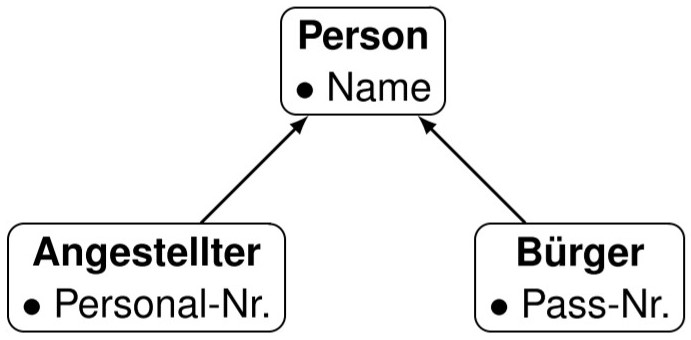
\includegraphics[width=0.8\linewidth]{images/v7_vererbung1}
\end{multicols}

\begin{itemize}
	\item Superklasse/Basisklasse:
	\item[\-] \lstinputlisting{listings/v7_vererbung1.py}
	\item Für die Vererbung: Superklasse in runden Klammern angeben
	\item Subklasse/abgeleitete Klasse:
	\item[\-] \lstinputlisting{listings/v7_vererbung2.py}
	\item Variablen und Methoden (\texttt{public} und \texttt{pretected}) werden direkt übernommen:
	\item[\-] \lstinputlisting{listings/v7_vererbung3.py}
	\item Methoden werden überschrieben, falls sie gleich heissen:
	\item[\-] \lstinputlisting{listings/v7_vererbung4.py}
	\item Zugriff auf die Superklasse mit \texttt{super()}
	\item[\-] \lstinputlisting{listings/v7_vererbung5.py}
\end{itemize}

\subsection{Beispiel}
\lstinputlisting{listings/v7_vererbung6.py}
Die Person-Klasse instanzieren:\\
\lstinputlisting{listings/v7_vererbung7.py}
Angestellte-Klasse erbt von der Person-Klasse:\\
\lstinputlisting{listings/v7_vererbung8.py}
Die Angestellter-Klasse instanzieren:\\
\lstinputlisting{listings/v7_vererbung9.py}

\subsection{\texttt{public}, \texttt{protected} und \texttt{private}}
Die Konvention ist wie folgt:
\begin{description}
	\item[\texttt{public:}] für für öffentliche Variablen und Methoden
	\item[\texttt{protected:}] (1 führender Unterstrich) für nicht-öffentliche Variablen und Methoden
	\item[\texttt{private:}] (2 führende Unterstriche) für nicht-öffentliche Variablen und Methoden, um Namenskonflikte in Subklassen zu vermeiden 
\end{description}
\url{https://www.python.org/dev/peps/pep-0008/#method-names-and-instance-variables}
\lstinputlisting{listings/v7_vererbung10.py}

\section{Mehrfachvererbung}
\begin{itemize}
	\item Eine Subklasse kann von mehreren Superklassen erben:
\end{itemize}
\begin{multicols}{2}
\lstinputlisting{listings/v7_vererbung11.py}
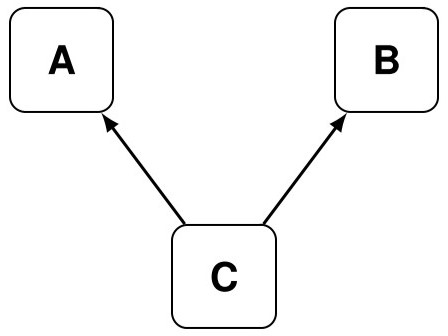
\includegraphics[width=0.7\linewidth]{images/v7_vererbung2}
\end{multicols}
Am besten die \texttt{\_init\_\(\)}-Methode der Klassen kooperativ machen, d.h.
\begin{itemize}
	\item immer \texttt{super()} benutzen
	\item Schlüsselwort-Argumente benutzen
	\item unbenutzte Schlüsselwort-Argumente weitergeben (\texttt{**kwargs})
\end{itemize}
\lstinputlisting{listings/v7_vererbung12.py}
\begin{multicols}{2}
\begin{itemize}
	\item \texttt{super()} ruft automatisch die Methode der nächsten Klasse auf
	\item Method Resolution Order (MRO) $\rightarrow$ C4 Superclass Linearization (\url{https://en.wikipedia.org/wiki/C3_linearizatio})
	\item Diamond-Problem ist kein Problem mit \texttt{super()}
\end{itemize}
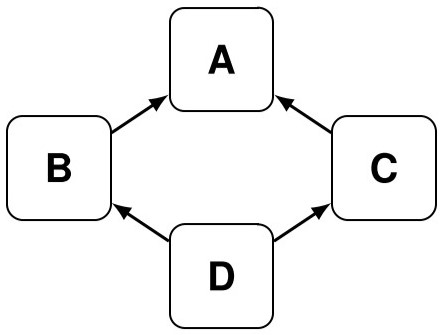
\includegraphics[width=0.5\linewidth]{images/v7_vererbung3}
\end{multicols}

\subsubsection{MRO}
Mehrfachvererbung in Diamant-Anordung:
\lstinputlisting{listings/v7_vererbung13.py}
\texttt{\textbf{super()}} ruft die Methoden der Reihe nach auf:
\lstinputlisting{listings/v7_vererbung14.py}
Die Reihenfolge wird vom MRO-Algorithmus festgelegt:
\lstinputlisting{listings/v7_vererbung15.py}

\part*{Lektion 8: NumPy und Matplotlib}
\section{NumPy}
\begin{itemize}
	\item Python-Bibliothek
	\item[\-] \texttt{import numpy as np}
	\item Einfache Handhabung mit Vektoren und Matrizen
	\begin{itemize}
		\item mehrdimensionale Arrays
	\end{itemize}
	\item Funktionen für numerische Berechnungen
	\begin{itemize}
		\item Grundlegende Operationen
		\item Mathematische Funktionen (sin, cos, sqrt, exp, ...)
		\item Lineare Algebra
		\item ...
	\end{itemize}
	\item Effiziente und schnelle Ausführung
	\begin{itemize}
		\item kompilierte Funktionen und Algorithmen
		\item Array-basierte Operationen $\rightarrow$ keine \texttt{for}-Schleifen
	\end{itemize}
	\item Ähnlichkeit zu MATLAB\textsuperscript{\textregistered}
	\item[\-] \url{https://docs.scipy.org/doc/numpy/user/ numpy-for-matlab-users.htm}
\end{itemize}

\subsection{ndarray erzeugen}
\begin{itemize}
	\item N-dimensionales Array (\url{https://docs.scipy.org/doc/numpy/reference/generated/numpy.ndarray.html})
	\item ndarray erzeugen\\
	\lstinputlisting{listings/v8_numpy1.py}
	\item Weitere Funktionen, um Arrays zu erzeugen\\
	\begin{tabular}{|l|l|}
		\hline 
		\textbf{Funktion} &\textbf{Resultat}\\ 
		\hline 
		\texttt{np.arange(3)} &\texttt{array([0, 1, 2])}\\ 
		\texttt{np.ones((2,2))} &\texttt{array([[1., 1.], [1., 1.]])}\\ 
		\texttt{np.ones\_like(arr1)} &\texttt{array([1, 1, 1])}\\ 
		\texttt{np.zeros((2,2))} &\texttt{array([[0., 0.], [0., 0.]])}\\ 
		\texttt{np.zeros\_like(arr1)} &\texttt{array([0, 0, 0])}\\ 
		\texttt{np.full((2,2), 7.0)} &\texttt{array([[7., 7.], [7., 7.]])}\\ 
		\texttt{np.full\_like(arr1, 7)} &\texttt{array([7, 7, 7])}\\ 
		\texttt{np.eye(2)} &\texttt{array([[1., 0.], [0., 1.]])}\\ 
		\texttt{np.identity(2)} &\texttt{array([[1., 0.], [0., 1.]])}\\ 
		\texttt{np.linspace(0, 1, 5)} &\texttt{array([0., 0.25, 0.5, 0.75, 1.])}\\ 
		\texttt{np.logspace(0, 1, 4)} &\texttt{array([1., 2.1544, 4.6416, 10.])}\\ 
		\texttt{np.random.randn(3)} &\texttt{array([0.7576, 0.0135, -0.8934])}\\ 
		\hline 
	\end{tabular} 
\end{itemize}

\subsubsection{ndarray-Datentypen}
\begin{itemize}
	\item Datentyp wird automatisch ermittelt,\\
	z.B. \texttt{np.int64} oder \texttt{np.float64}
	\item Datentyp erzwingen\\
	\texttt{np.array([1, 2, 3], dtype=np.complex)}
	\item Mögliche Datentypen\\
	\begin{tabular}{|l|l|}
		\hline 
		\texttt{np.int8, np.uint8} &8-Bit Ganzzahlen\\ 
		\texttt{np.int16, np.uint16} &16-Bit Ganzzahlen\\ 
		\texttt{np.int32, np.uint32} &32-Bit Ganzzahlen\\ 
		\texttt{np.int64, np.uint64} &64-Bit Ganzzahlen\\ 
		\texttt{np.float16} &Float mit halber Genauigkeit\\ 
		\texttt{np.float32} &Float mit einfacher Genauigkeit\\ 
		\texttt{np.float64} &Float mit doppelter Genauigkeit\\ 
		\texttt{np.float128} &Float mit vierfacher Genauigkeit\\  
		\texttt{np.complex64/128/256} &Komplexe Zahl\\ 
		\texttt{np.bool} &Boolescher Wert, True/False\\ 
		\hline 
	\end{tabular} 
\end{itemize}

\subsection{Arithmetische Operationen}
\begin{itemize}
	\item Arithmetische Operationen werden elementweise ausgeführt\\
	\lstinputlisting{listings/v8_numpy2.py}
	\begin{tabular}{|l|l|}
		\hline
		\textbf{Operation} &\textbf{Resultat}\\
		\hline
		\texttt{arr + arr} &\texttt{array([2., 4., 6.])}\\
		\texttt{arr + 1} &\texttt{array([2., 3., 4.])}\\
		\texttt{arr - arr} &\texttt{array([0., 0., 0.])}\\
		\texttt{arr - 1} &\texttt{array([0., 1., 2.])}\\
		\texttt{arr*arr} &\texttt{array([1., 4., 9.])}\\
		\texttt{arr*2} &\texttt{array([2., 4., 6.])}\\
		\texttt{arr/arr} &\texttt{array([1., 1., 1.])}\\
		\texttt{arr/2} &\texttt{array([0.5, 1., 1.5])}\\
		\texttt{arr**2} &\texttt{array([1., 4., 9.])}\\
		\texttt{arr > 2} &\texttt{array([False, False, True], dtype=bool)}\\
		\hline
	\end{tabular}
\end{itemize}

\vfill\null
\pagebreak
\subsection{Indexierung}
\begin{multicols}{2}
	\begin{itemize}
		\item Indexierung von 2D-Arrays\\
		\lstinputlisting{listings/v8_numpy3.py}
		\item Beispiele:\\
		\lstinputlisting{listings/v8_numpy4.py}
	\end{itemize}
	\columnbreak
	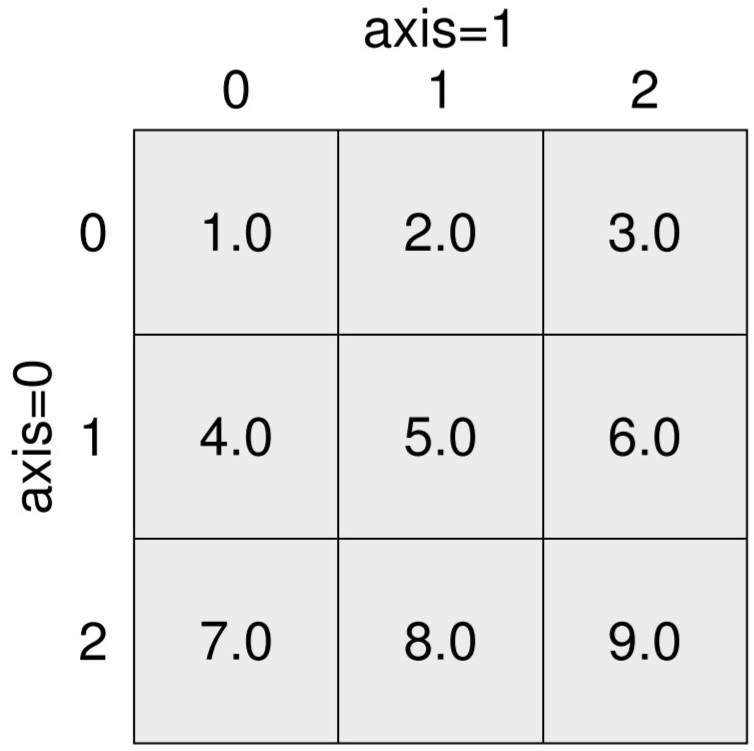
\includegraphics[width=0.7\linewidth]{images/v8_numpy1}
\end{multicols}

\subsubsection{Slicing}
\begin{tabular}{|l|l|l|l|}
	\hline
	\texttt{arr} &Ausdruck &Shape &Resultat\\
	\hline
	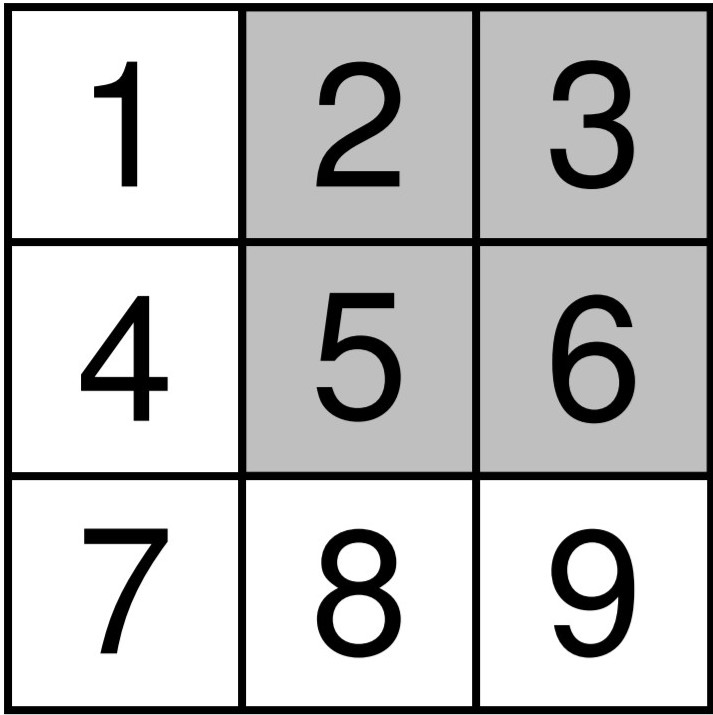
\includegraphics[width=0.1\linewidth]{images/v8_numpy2} &\texttt{arr[:2, 1:]} &(2,2) &\texttt{array([[2, 3], [5, 6]])}\\
	\hline
	\multirow{3}{0.1\linewidth}{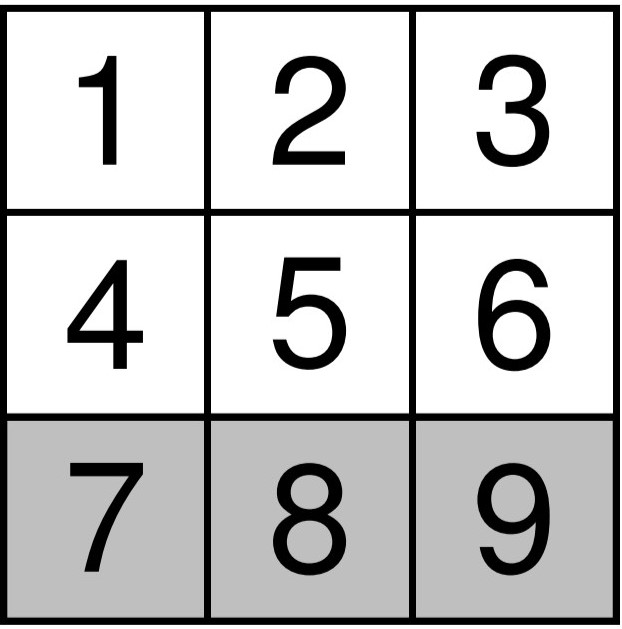
\includegraphics[width=\linewidth]{images/v8_numpy3}} &\texttt{arr[2]} &(3, ) &\texttt{array([7, 8, 9])}\\
	&\texttt{arr[2, :]} &(3, ) &\texttt{array([7, 8, 9])}\\
	&\texttt{arr[2:, :]} &(1, 3) &\texttt{array([[7, 8, 9]])}\\
	\hline
	\multirow{3}{0.1\linewidth}{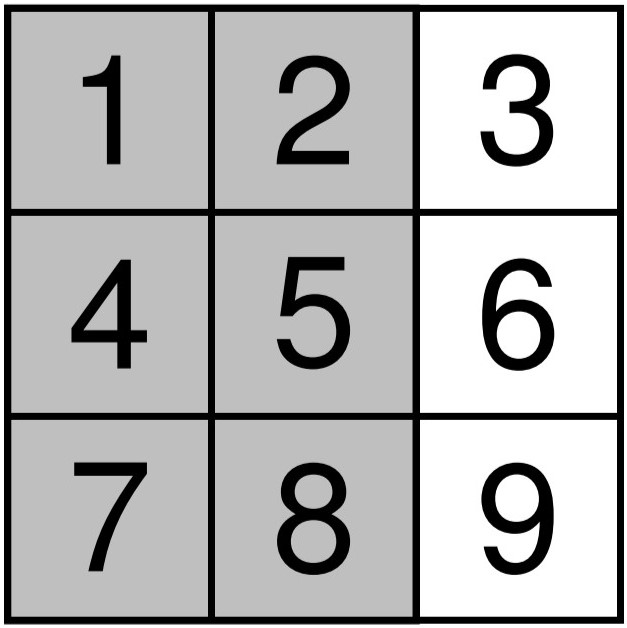
\includegraphics[width=\linewidth]{images/v8_numpy4}} &\texttt{arr[:, :2]} &(3, 2) &\texttt{array([[1, 2],}\\
	& & &\texttt{[4, 5],}\\
	& & &\texttt{[7, 8]])}\\
	\hline
	\multirow{3}{0.1\linewidth}{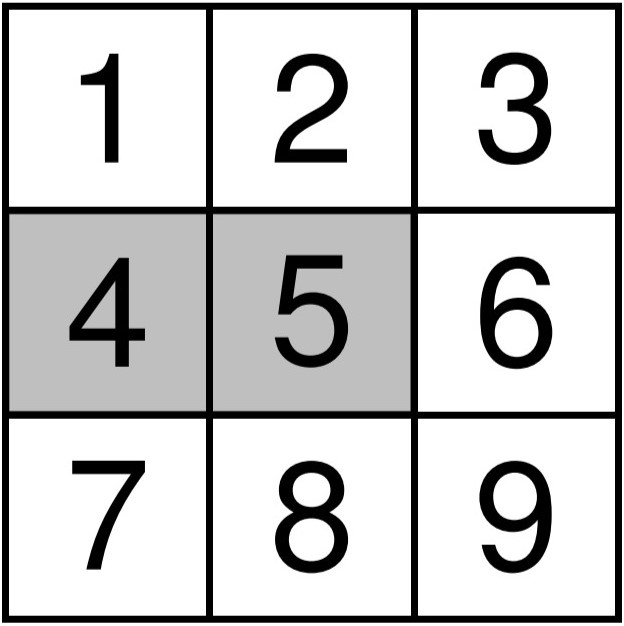
\includegraphics[width=\linewidth]{images/v8_numpy5}} &\texttt{arr[1, :2]} &(2, ) &\texttt{array([4, 5])}\\
	&\texttt{arr[1:2, :2]} &(1, 2) &\texttt{array([[4, 5]])}\\
	& & &\\
	\hline
\end{tabular}\\
$\rightarrow$ \texttt{ndim} bleibt erhalten, falls bei jeder \texttt{axis} ein $"$:$"$ steht.
\begin{itemize}
	\item Ein Slice ist immer eine Referenz, keine Kopie!
	\lstinputlisting{listings/v8_numpy5.py}
	\item Kopien werden mit \texttt{.copy()} erzeugt:
	\lstinputlisting{listings/v8_numpy6.py}
	\item Zuweisung eines Skalars zu einem Slice wird ausgebreitet:
	\lstinputlisting{listings/v8_numpy7.py}
	\item Bei fehlender Dimension wird das Array automatisch erweitert:
	\lstinputlisting{listings/v8_numpy8.py}
\end{itemize}
$\rightarrow$ Bedingung: letzte Dimension ist gleich oder nur 1 lang.

\subsection{Mathematische Funktionen}
\begin{itemize}
	\item NumPy beinhaltet viele mathematische Funktionen:\\
	\url{https://docs.scipy.org/doc/numpy/reference/routines.math.html}
	\begin{itemize}
		\item \texttt{np.sin()}
		\item \texttt{np.cos()}
		\item \texttt{np.exp()}
		\item \texttt{np.cumsum()}
		\item ...
	\end{itemize}
	\item Diese Funktionen operieren über das gesamte Array
	\lstinputlisting{listings/v8_numpy9.py}
\end{itemize}

\subsubsection{Lineare Algebra}
\begin{itemize}
	\item Liste der Funktionen:\\
	\url{https://docs.scipy.org/doc/numpy/reference/routines.linalg.html}
	\item Matrix definieren
	\lstinputlisting{listings/v8_numpy14.py}
	\item Vektor definieren
	\lstinputlisting{listings/v8_numpy15.py}
	\item Matrix \textbf{M} mit Vektor \textbf{v} multiplizieren
	\lstinputlisting{listings/v8_numpy10.py}
	\item Matrix transponieren \textbf{M$^T$}
	\lstinputlisting{listings/v8_numpy11.py}
	\item Matrix invertieren \textbf{M$^{-1}$}
	\lstinputlisting{listings/v8_numpy12.py}
	\item Shape eines Vektors ändern
	\lstinputlisting{listings/v8_numpy16.py}
\end{itemize}

\subsubsection{Matplotlib}
\begin{itemize}
	\item Python-Bibliothek\\
	\texttt{import matplotlib.pyplot as plt}
	\item Erstellen von publizierbaren Diagrammen und Darstellungen
	\item 100\% kompatibel zu NumPy-Arrays
	\item MATLAB\textsuperscript{\textregistered}-ähnliche Funktionen:\\
	\url{https://matplotlib.org/api/_as_gen/matplotlib.pyplot.html}
	\item Kann auch objekt-orientiert verwendet werden, z.B. in GUIs
	\item Grosse Beispiel-Sammlung:\\
	\url{https://matplotlib.org/gallery/index.html}
	\item Einfaches Beispiel:
\end{itemize}
\begin{multicols}{2}
	\lstinputlisting{listings/v8_numpy13.py}
	\vfill\null
	\columnbreak
	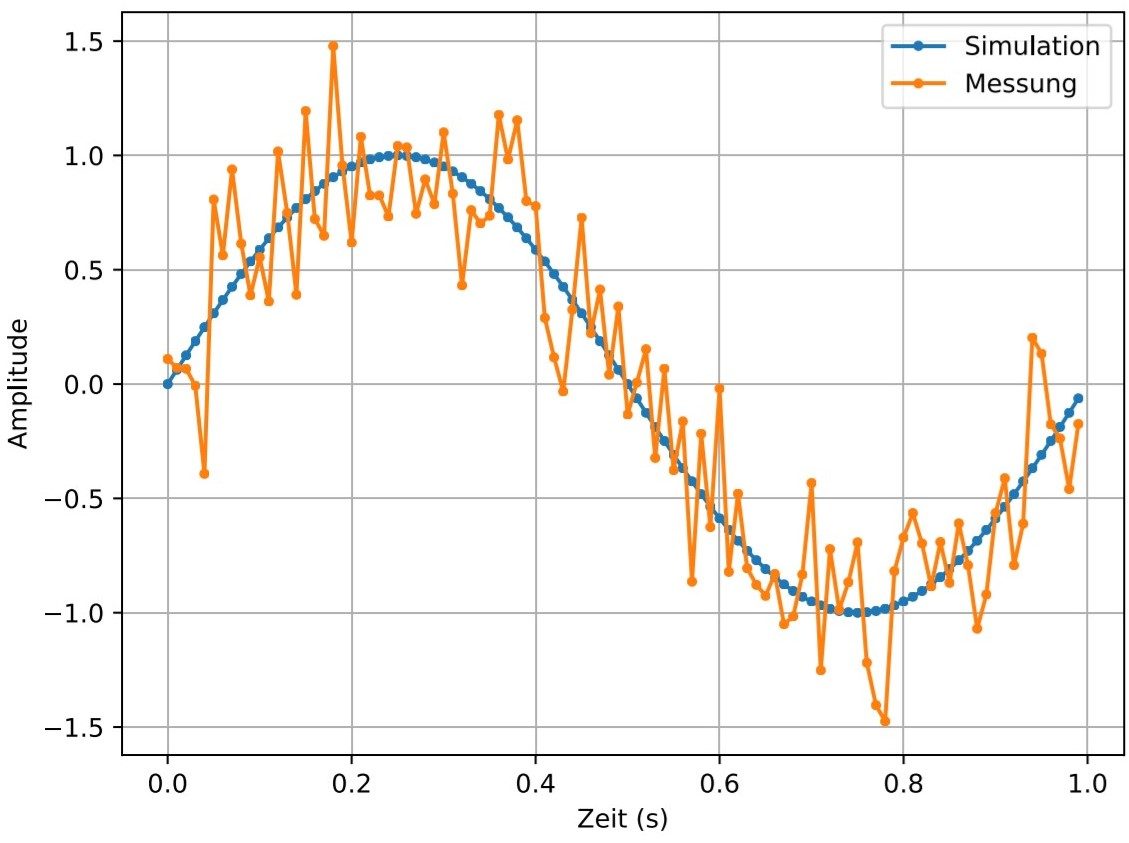
\includegraphics[width=\linewidth]{images/v8_numpy6}
\end{multicols}
\section{SciPy}
\begin{itemize}
	\item Python-Bibliothek
	\item[\-] \texttt{from scipy import integrate, interpolate, optimize, signal, ...}
	\item Basiert auf NumPy
	\item Enthält numerische Algorithmen und mathematische Werkzeuge\\
	\item \url{https://docs.scipy.org/doc/scipy/reference/}
\end{itemize}

\begin{minipage}[t]{0.49\textwidth}
	\subsection{SciPy.Interpolate}
	\begin{itemize}
		\item 1-dimensionale Interpolation
		\item Mehrdimensionale Interpolation
		\item Splines
		\item API-Referenz: \url{https://docs.scipy.org/doc/scipy/reference/interpolate.html}
	\end{itemize}
\end{minipage}
\hspace{0.02\textwidth}
\begin{minipage}[t]{0.49\textwidth}
	\lstinputlisting{listings/v9_interpolate1.py}
	Stützwerte für x und y:
	\lstinputlisting{listings/v9_interpolate2.py}
\end{minipage}\\[12pt]

\begin{minipage}[t]{0.54\textwidth}
	Interpolationsfunktionen erstellen:
	\lstinputlisting{listings/v9_interpolate3.py}
\end{minipage}
\hspace{0.02\textwidth}
\begin{minipage}[t]{0.44\textwidth}
	$\quad$\\[1pt]
	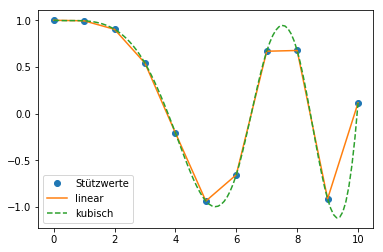
\includegraphics[width=\textwidth]{images/v9_interpolate1}
\end{minipage}




\subsection{SciPy.Integrate}
\begin{itemize}
	\item Integration von gegebenen Funktionen
	\item Integration von diskreten Samples
	\item Numerische Integratoren für Differentialgleichungen (ODE)
	\item API-Referenz: \url{https://docs.scipy.org/doc/scipy/reference/integrate.html}
\end{itemize}

\begin{minipage}[t]{0.49\textwidth}
	Diskrete Samples:
	\lstinputlisting{listings/v9_integrate2.py}
\end{minipage}
\hspace{0.02\textwidth}
\begin{minipage}[t]{0.49\textwidth}
	$\quad$\\[1pt]
	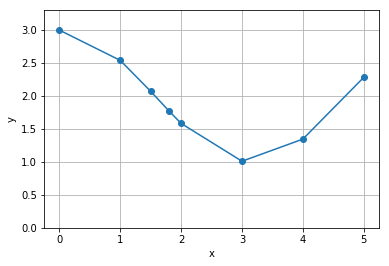
\includegraphics[width=\textwidth]{images/v9_integrate1}
\end{minipage}

\begin{minipage}[t]{0.49\textwidth}
	$\quad$\\[15pt]
	Integral (Fläche unter dem Graphen) berechnen:
\end{minipage}
\hspace{0.02\textwidth}
\begin{minipage}[t]{0.49\textwidth}
	\lstinputlisting{listings/v9_integrate3.py}
\end{minipage}


\pagebreak

\textbf{Gegebene Funktion}
\lstinputlisting{listings/v9_integrate4.py}

\section{Matplotlib}
\begin{itemize}
%	\item Tipps und Tricks in Jupyter
	\item Figure mit Subplots erstellen
	\item \texttt{plt.contour()} und \texttt{plt.contourf()}
	\item \texttt{plt.loglog()}
\end{itemize}

%\subsection{Tipps für Jupyter-Notebook}
%Folgende Zeile einfügen, damit man nicht immer \texttt{plt.show()} aufrufen muss
%\lstinputlisting{listings/v9_matplotlib1.py}
%Ein Semikolon am Zeilenende unterdrückt lästige Meldungen (\texttt{plt.plot(...);})

\subsection{Subplots}
\begin{minipage}[t]{0.49\textwidth}
	Einzelne Subplots nacheinander erstellen:
	\lstinputlisting{listings/v9_matplotlib2.py}
\end{minipage}
\hspace{0.02\textwidth}
\begin{minipage}[t]{0.49\textwidth}
	Alle Subplots von Anfang an erstellen:
	\lstinputlisting{listings/v9_matplotlib3.py}
	
\end{minipage}


\begin{minipage}[t]{0.49\textwidth}
	\subsection{Pyplot-Funktionen}
	\subsubsection{Treppensignal}
	\lstinputlisting{listings/v9_matplotlib4.py}
\end{minipage}
\hspace{0.02\textwidth}
\begin{minipage}[t]{0.49\textwidth}
	$\quad$\\[1pt]
	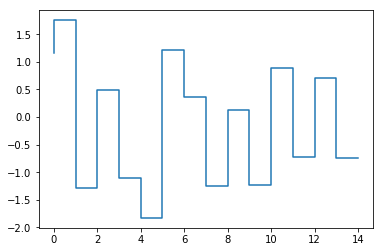
\includegraphics[width=0.8\textwidth]{images/v9_matplotlib1}
\end{minipage}

	\subsubsection{\texttt{contourf()}}
\url{https://matplotlib.org/api/_as_gen/matplotlib.pyplot.contourf.html}\\
\url{https://matplotlib.org/tutorials/colors/colormaps.html}\\
\begin{minipage}[t]{0.54\textwidth}
	\lstinputlisting{listings/v9_matplotlib5.py}
\end{minipage}
\hspace{0.02\textwidth}
\begin{minipage}[t]{0.44\textwidth}
	$\quad$\\[1pt]
	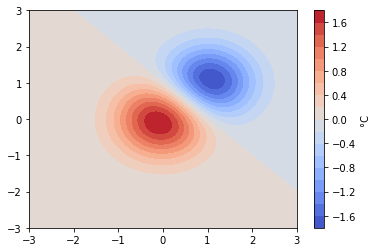
\includegraphics[width=0.9\textwidth]{images/v9_matplotlib2}
\end{minipage}




\subsubsection{\texttt{contour()}}
\url{https://matplotlib.org/api/_as_gen/matplotlib.pyplot.contour.html}\\
\begin{minipage}[t]{0.49\textwidth}
	\lstinputlisting{listings/v9_matplotlib6.py}
\end{minipage}
\hspace{0.02\textwidth}
\begin{minipage}[t]{0.49\textwidth}
	$\quad$\\[1pt]
	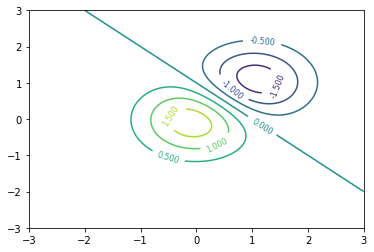
\includegraphics[width=0.75\textwidth]{images/v9_matplotlib3}
\end{minipage}


\subsubsection{\texttt{loglog()}}
\url{https://matplotlib.org/api/_as_gen/matplotlib.pyplot.loglog.html}\\
\begin{minipage}[t]{0.49\textwidth}
	\lstinputlisting{listings/v9_matplotlib7.py}
\end{minipage}
\hspace{0.02\textwidth}
\begin{minipage}[t]{0.49\textwidth}
	$\quad$\\[1pt]
	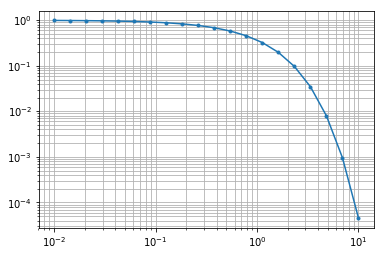
\includegraphics[width=0.75\textwidth]{images/v9_matplotlib4}
\end{minipage}




\subsubsection{XKCD}
\url{https://xkcd.com/}\\
\url{https://matplotlib.org/api/_as_gen/matplotlib.pyplot.xkcd.html}\\
\url{https://packages.debian.org/buster/fonts-humor-sans}\\
\url{https://github.com/shreyankg/xkcd-desktop/blob/master/Humor-Sans.ttf}\\
\begin{minipage}[t]{0.49\textwidth}
	\lstinputlisting{listings/v9_matplotlib8.py}
\end{minipage}
\hspace{0.02\textwidth}
\begin{minipage}[t]{0.49\textwidth}
	$\quad$\\[1pt]
	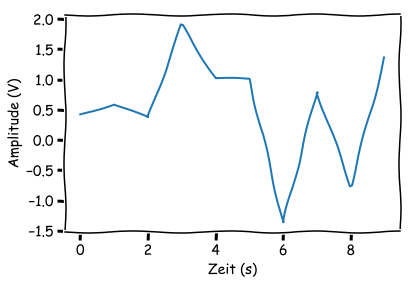
\includegraphics[width=0.75\textwidth]{images/v9_matplotlib5}
\end{minipage}


\end{document}
